%%%%%%%%%%%%%%%%%%%%%%%%%%%%%%%%%%%%%%%%%%%%%%%%%%%%%%%%%%%%%%%%%%%%%%%%%%%%%%%%%%%%%%%%%%
%%%%%%%%%%%%
%%%%%%%%%%%% This report template was constructed by
%%%%%%%%%%%% Fredrik Hedström & Jörg Schminder, Linköping university, 2016
%%%%%%%%%%%% and correspond to LiU's official layout for Master-These reports. 
%%%%%%%%%%%%
%%%%%%%%%%%%%%%%%%%%%%%%%%%%%%%%%%%%%%%%%%%%%%%%%%%%%%%%%%%%%%%%%%%%%%%%%%%%%%%%%%%%%%%%%%

\documentclass[11pt,a4paper,twoside,oneside]{article}

    %\usepackage{fontspec}
    %\setmainfont{Calibri} 

\usepackage{mystyle}



%\defaultbibliography{references.bib}
%\defaultbibliographystyle{vancouver}

\begin{document}
%\begin{bibunit}[plain]
%%%%%%%%%%%%%%%%%%%%%%%%%%%%%%%%%%%%%%%%%%%%%%%%%%%%%%%%%%%%%%%%%%%%%%%%%%%%%%%%%%%%%%%%%%
%%%%%%%%%%%%
%%%%%%%%%%%%    											Title page 1
%%%%%%%%%%%%
%%%%%%%%%%%%%%%%%%%%%%%%%%%%%%%%%%%%%%%%%%%%%%%%%%%%%%%%%%%%%%%%%%%%%%%%%%%%%%%%%%%%%%%%%%
\begin{titlepage}

\newgeometry{left=1.5cm, right=1.5cm, top=1.4cm, bottom=.9cm} 	
    \hfill
    \begin{minipage}{15cm}
        \begin{onehalfspacing}
        \raggedleft
        Link\"opings universitet\\
        Institutionen f\"or ekonomisk och industriell utveckling\\
        Department of Applied Thermodynamics and Fluid Mechanics \\
        Master Thesis 2021\\%$|$LIU-IEI-XXX-YY/XXXXX-SE \\
        LIU-IEI-TEK-A--21/04226-SE\\
        \end{onehalfspacing}
    \end{minipage}
    
	\vspace{2cm}
	\noindent
	\hspace{3cm} 
	{\Huge\textbf{CFD Simulation of a\\
	\hspace*{3.1cm}Fin-Tube evaporator\\
	\hspace*{3.1cm}under icing}\par}
	
% 	\vspace{1cm}
% 	\noindent \hspace{3cm} 
% 	{\Large\textbf{And a possible subtitle could be positioned here} \par}
	
	\vspace{.5cm}
	\noindent
	\hspace{3cm}
	\hrulefill
	\hspace{2.7cm}
	
	\vspace{1.3cm}
	\noindent \hspace{3cm}{\large \textbf{Abhay Mahesh Hervatte (abhhe344)}}

%   \vspace{0.3cm}
%   \noindent \hspace{3cm}{\large \textbf{Author Name (Nr2)}}
	
    \vspace{1.2cm}
    \noindent \hspace{3cm}{{\large Academic supervisor: Johan Renner \par}
    \noindent \hspace{2.88cm} {\large Industrial supervisors: Yuting Tan, Alister Clay  \par}
    \noindent \hspace{2.88cm} {\large Examiner: Roland G\aa rdhagen \par}}
    
    \begin{center}
        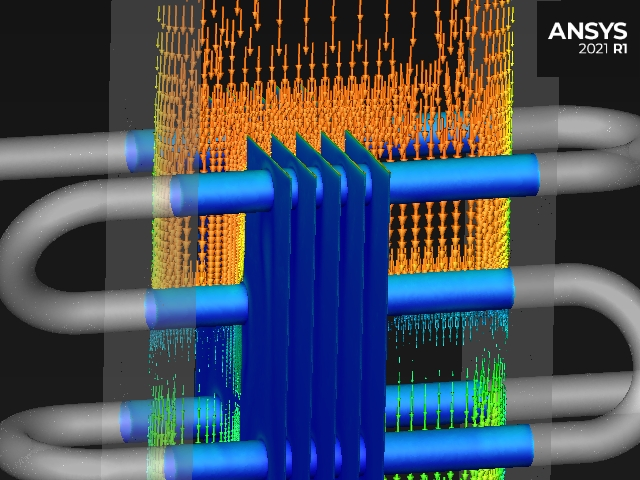
\includegraphics[width=0.8\textwidth]{images/resss/640480.jpg}	
    \end{center}
    
    \vfill
    
    \noindent
    \begin{minipage}{6.2cm}
    \hspace{.45cm} \includegraphics*[width=6.2cm]{LiuLogo.eps}
    \end{minipage}\hfill
    \begin{minipage}{9cm}
        \begin{onehalfspacing}
        \raggedleft
        Link\"oping University\\
        SE-581 83 Link\"oping, Sverige\\
        013-28 10 00, www.liu.se \\
        \end{onehalfspacing}
    \end{minipage}
    
\end{titlepage}

%%%%%%%%%%%%%%%%%%%%%%%%%%%%%%%%%%%%%%%%%%%%%%%%%%%%%%%%%%%%%%%%%%%%%%%%%%%%%%%%%%%%%%%%%%
%%%%%%%%%%%%
%%%%%%%%%%%%    											Title page 2
%%%%%%%%%%%%
%%%%%%%%%%%%%%%%%%%%%%%%%%%%%%%%%%%%%%%%%%%%%%%%%%%%%%%%%%%%%%%%%%%%%%%%%%%%%%%%%%%%%%%%%%
\cleardoublepage
\thispagestyle{empty}
\begin{titlepage}
\newgeometry{left=1.5cm, right=1.5cm, top=0cm, bottom=.9cm} 
	\vspace*{2.5cm}
	\noindent \hspace{3.3cm} 
	{\Huge\textbf{CFD Simulation of a\\
	\hspace*{3.4cm}Fin-Tube evaporator\\
	\hspace*{3.4cm}under icing}\par}
	
% 	\vspace{1cm}
% 	\noindent \hspace{3.5cm} 
% 	{\Large\textbf{And a possible subtitle could be positioned here} \par}
	
	\vspace{1.6cm}
	\noindent \hspace{3.7cm}{\large \textbf{Abhay Mahesh Hervatte (abhhe344)}}
	
% 	\vspace{0.3cm}
%   \noindent \hspace{3.7cm}{\large \textbf{Author Name (Nr2)}}
		
\vspace{7cm}
  \noindent \hspace{5.5cm}%{\large \textit{A possible picture could be positioned here}}
    \begin{center}
        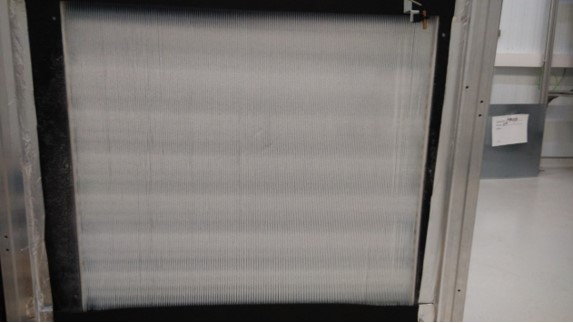
\includegraphics[width=0.8\textwidth]{images/Picture1.jpg}	
    \end{center}
    \vfill
    \noindent
		
    \begin{minipage}{6.2cm}
    \includegraphics*[width=6.9cm]{LiuLogo.eps}
    \end{minipage}\hfill
    \begin{minipage}{9cm}
    \begin{onehalfspacing}
        \raggedleft
        Link\"opings universitet\\
        Institutionen f\"or ekonomisk och industriell utveckling\\
        Master Thesis 2021\\%$|$LIU-IEI-XXX-YY/XXXXX-SE \\
        LIU-IEI-TEK-A--21/04226-SE\\
        \end{onehalfspacing}
    \end{minipage}
 \restoregeometry

\end{titlepage}


%%%%%%%%%%%%%%%%%%%%%%%%%%%%%%%%%%%%%%%%%%%%%%%%%%%%%%%%%%%%%%%%%%%%%%%%%%%%%%%%%%%%%%%%%%
%%%%%%%%%%%%
%%%%%%%%%%%%    											Abstract
%%%%%%%%%%%%
%%%%%%%%%%%%%%%%%%%%%%%%%%%%%%%%%%%%%%%%%%%%%%%%%%%%%%%%%%%%%%%%%%%%%%%%%%%%%%%%%%%%%%%%%%

\cleardoublepage
\thispagestyle{plain}
\pagenumbering{roman}

\section*{Abstract}

\vspace{.6cm}

The study involves development of a methodology to simulate a fin-tube evaporator under icing conditions using CFD in \emph{Ansys{\textregistered} Academic Fluent 2021R1}\cite{flug}. It aims to build on previous studies performed on heat pumps. It was performed by Abhay M. Hervatte in collaboration with Bosch Thermoteknik AB, Tran\aa s, SE during the spring term of the year 2021. The thesis is published by Link\"oping University.

Initially, experiments were conducted to measure the ice growth on the fins of the evaporator as a function of time. A CAD model of the evaporator was then generated. The evaporator geometry was scaled down and simplified in order to reduce the simulation time. Due to restrictions in the software, the simulations were split into two parts - one for the flow of the refrigerant through the evaporator pipes and another for flow of air over the fins. The internal flow simulation was a steady state simulation consisting of the phase-change of the refrigerant after absorbing heat from the ambient. through the pipes and a transient simulation for the external flow over the fins. The internal flow consisted of multi-phase simulation of the evaporation of the refrigerant - propane - after absorbing heat through the pipe walls. The external flow involved the multi-phase simulation of ice being deposited from humid air on the surface of the fins. The inner surface of the evaporator pipes was used as a bridge, and surface profiles from the internal simulation would be used to transfer the boundary conditions to the other simulation. Results of the ice-film thickness over the fins were obtained and compared to the experimental value and found to be in reasonable agreement with each other, with scope for improvement in the future.

%%%%%%%%%%%%%%%%%%%%%%%%%%%%%%%%%%%%%%%%%%%%%%%%%%%%%%%%%%%%%%%%%%%%%%%%%%%%%%%%%%%%%%%%%%
%%%%%%%%%%%%
%%%%%%%%%%%%    											Acknowledgements
%%%%%%%%%%%%
%%%%%%%%%%%%%%%%%%%%%%%%%%%%%%%%%%%%%%%%%%%%%%%%%%%%%%%%%%%%%%%%%%%%%%%%%%%%%%%%%%%%%%%%%%
\cleardoublepage

\thispagestyle{plain}

\section*{Acknowledgements}

\vspace{.6cm}

I would like to start by dedicating my Master's Thesis in memory of my father Mahesh Hervatte, without whose belief in me, I wouldn't have been able to pursue a master's degree, let alone this thesis. Thank you for everything, pa.\\

I would like to take this opportunity thank my supervisors Yuting Tan at Bosch and Prof. Johan Renner, Link\"oping University, and my examiner Prof. Roland G\aa rdhagen, Link\"oping University for their continued support through the course of my Master's Thesis. I would also like to thank my team manager, Victor Fransson at Bosch for giving me this opportunity and making me a part of the team. I also want to thank the entire RHP-ERM team at Bosch Tran\aa s for welcoming me.\\

I would like to thank Sebastian Grudemo for his help with the CAD aspects of my thesis. I want to also thank Alister Clay at Bosch, Wernau for his help with fine-tuning the CFD. His guidance and support was present at all times during my thesis and was an integral part of successfully completing my work as assigned. His expertise in the subject definitely proved helpful whenever there were problems during the thesis work.\\

I also want to extend my gratitude to my colleagues at Link\"oping University, Sadegh Fattahi and Anton Persson for their help at a few critical junctures during the development of the methodology. They were able to provide key insights that helped me think outside the box to find a few solutions. My coursemates Kevin Swamy, Pranav Rane and Avi Bhambhani were integral partners  during the course of my studies at Link\"oping University, without whom this thesis would have been a lot more difficult to complete.\\

Last but not least, I want to extend my sincere thanks and gratitude to my mother Sadhana Hervatte for believing in me, supporting me and helping me navigate the ups and downs of life.\\

Images courtesy of Ansys Inc.
\begin{figure*}[!ht]
    \centering
    \begin{subfigure}{0.4\textwidth}
    
\includegraphics[width=0.99\textwidth]{images/bosch.png}
    \end{subfigure}
    \begin{subfigure}{0.4\textwidth}
    
\includegraphics[width=0.99\textwidth]{images/anslogo.png}
    \end{subfigure}
    % \caption{Caption}
    % \label{fig:my_label}
\end{figure*}
%%%%%%%%%%%%%%%%%%%%%%%%%%%%%%%%%%%%%%%%%%%%%%%%%%%%%%%%%%%%%%%%%%%%%%%%%%%%%%%%%%%%%%%%%%
%%%%%%%%%%%%
%%%%%%%%%%%%    											Nomenclature
%%%%%%%%%%%%
%%%%%%%%%%%%%%%%%%%%%%%%%%%%%%%%%%%%%%%%%%%%%%%%%%%%%%%%%%%%%%%%%%%%%%%%%%%%%%%%%%%%%%%%%%

\cleardoublepage

\thispagestyle{plain}

\section*{Nomenclature}

\vspace{.6cm}


\vspace{-2ex}
\subsubsection*{Acronyms}

\vspace*{-2ex}

\begin{longtable}{p{.25\textwidth}p{.65\textwidth}} % Abbreviations
  \hline
  \multicolumn{1}{l}{\bfseries Acronym} &
  \multicolumn{1}{l}{\bfseries Expansion}\\
  \hline
\endhead
  \hline
\endfoot

LiU     & Link\"oping University\\
CFD			& Computational fluid dynamics\\
CAD     & Computer aided design\\
CPU 		& Central processing unit\\
RGP & Real Gas Property\\
RMS & Root Mean Square\\
UDF & User Defined Function\\
EWF & Eulerian Wall Film\\


\end{longtable}

\vspace*{1ex}

\subsubsection*{Latin Symbols}

\vspace*{-2ex}

\setlength\extrarowheight{1pt}
\begin{longtable}{>{$\displaystyle$}p{.20\textwidth}>{}p{.46\textwidth}>{}p{.23\textwidth}}
	\hline
  \multicolumn{1}{l}{\bfseries Symbol} &
  \multicolumn{1}{l}{\bfseries Description} &
	\multicolumn{1}{l}{\bfseries Units} \\
  \hline
\endhead
  \hline
\endfoot

A  & area 	& $\left[m^{2}\right]$\\
$\Delta P$ & Pressure Difference & $\left[Pa\right]$\\
$p$     & Static Pressure             & $[Pa]$        \\ 
$g$      & Acceleration due to Gravity & $[m s^{-2}]$  \\ 
$\vec{v}$                    & Velocity Vector & $[m s^{-1}]$         \\
$\mu$                        & Dynamic Viscosity                & $[N s m^{-2}]$ \\
$k$                          & Turbulent Kinetic Energy         & $[m^2s^{-2}]$  \\
$T$                          & Temperature                      & $[K]$          \\
$Sc_t$                       & Turbulent Schmidt Number         & $[-]$          \\
$\dot{m}$                    & Mass flow rate                   & $[kg s^{-1}]$  \\

% c 												& heat capacity						& $\left[W m^{-2} K^{-1}\right]$\\
% $\vec n$ 										& Normal vector						& $\left[-\right]$\\
% p 												& Pressure								& $\left[Pa\right]$\\
% t 												& Time										& $\left[s\right]$\\

\end{longtable} 

\vspace*{1ex}

\subsubsection*{Greek Symbols}

\vspace*{-2ex}

\setlength\extrarowheight{1pt}
\begin{longtable}{>{$\displaystyle$}p{.20\textwidth}>{}p{.46\textwidth}>{}p{.23\textwidth}} % Math | p{.25\textwidth} | p{.25\textwidth}| p{.25\textwidth} | p{.25\textwidth}|
	\hline
  \multicolumn{1}{l}{\bfseries Symbol} &
  \multicolumn{1}{l}{\bfseries Description} &
	\multicolumn{1}{l}{\bfseries Units} \\
  \hline
\endhead
  \hline
\endfoot

$\lambda$ & Flow Head & $[-]$\\
$\overline{\overline{\tau}}$ & Stress Tensor                    & $[Nm^{-2}]$    \\
$\epsilon$                   & Rate of Dissipation of $k$       & $[m^2s^{-3}]$  \\
$\omega$                     & Specific Dissipation Rate of $k$ & $[s^{-1}]$     \\
$\alpha$                     & Volume Fraction                  & $[-]$          \\
$\rho$ & Density                     & $[kg m^{-3}]$ \\

% $\alpha$ 									& Angle																	& $\left[degree\right]$\\
% $\mu $										& Dynamics viscosity										& $\left[kg m^{-1} s^{-1}\right]$\\
% $\Pi_{ij}$ 								& Pressure-velocity gradient tensor			& $\left[m^{2} s^{-3}\right]$\\

\end{longtable} 

\vspace*{1ex}


% \subsubsection*{Subscripts and superscripts}
% \vspace*{-2ex}

% \begin{longtable}{p{.25\textwidth}p{.65\textwidth}} % Abbreviations
%   \hline
%   \multicolumn{1}{l}{\bfseries Abbreviation} &
%   \multicolumn{1}{l}{\bfseries Meaning}\\
%   \hline
% \endhead
%   \hline
% \endfoot

% i		    	& running number\\
% bla				& arterial blood \\
% 0       	& sign of neutrality\\
% $\infty$ 	& sign of environment\\

% \end{longtable}

%%%%%%%%%%%%%%%%%%%%%%%%%%%%%%%%%%%%%%%%%%%%%%%%%%%%%%%%%%%%%%%%%%%%%%%%%%%%%%%%%%%%%%%%%%
%%%%%%%%%%%%
%%%%%%%%%%%%    											Table of content
%%%%%%%%%%%%
%%%%%%%%%%%%%%%%%%%%%%%%%%%%%%%%%%%%%%%%%%%%%%%%%%%%%%%%%%%%%%%%%%%%%%%%%%%%%%%%%%%%%%%%%%
\cleardoublepage

\thispagestyle{plain}

\tableofcontents
\listoffigures
\listoftables
%%%%%%%%%%%%%%%%%%%%%%%%%%%%%%%%%%%%%%%%%%%%%%%%%%%%%%%%%%%%%%%%%%%%%%%%%%%%%%%%%%%%%%%%%%
%%%%%%%%%%%%
%%%%%%%%%%%%    											Theses
%%%%%%%%%%%%
%%%%%%%%%%%%%%%%%%%%%%%%%%%%%%%%%%%%%%%%%%%%%%%%%%%%%%%%%%%%%%%%%%%%%%%%%%%%%%%%%%%%%%%%%%



%%%%%%%%%%%%%%%%%%%%%%%%%%%%%%%%  Chapter 1  %%%%%%%%%%%%%%%%%%%%%%%%%%%%%%%%%%%%%%%%%%%
\cleardoublepage

\thispagestyle{plain}

\pagenumbering{arabic}
\onehalfspacing
\section{Introduction}
\vspace{.6cm}

%%Add something about project eg: This is a master thesis proj about hp and so on, at Bosch. Broad sense of report. 4-5 sentences
This {report} is done as a part of the master's thesis as part of the degree in Aeronautical Engineering. It was conducted in collaboration with Bosch Thermoteknik AB, Tran\aa s Sweden regarding their heat pump testing system. The study is a way for the company to obtain a working simulation model of a heat pump that can predict the behaviour of new heat pumps without the need to build a prototype and test it. This report showcases the methodology that was followed in order to obtain a preliminary model for the heat pump {evaporator} under icing conditions.

Heat pumps are integral to homes in cold climates such as Sweden. They are  devices that absorb energy from a cold region (i.e. the external environment) and release it into a warmer home/room. There are different types of heat pumps that perform this function in different ways, as shown\textsuperscript{\cite{hundybook}}:
\begin{itemize}
    \item \textbf{Ground Source Heat Pumps (GSHP)}: Use water (ideally geothermal/hot water) as the source of heating, where water (with antifreeze) passes through the circuit which is submerged in the waterbody. Based on the source of the heat, these can be specifically categorized under "Water Source" or "Geothermal Source" heat pumps. Since the temperature underground remains relatively stable (similar to the bottom of lakes/other large bodies of water), these pumps have a source temperature of 5-10$\degree C$. Additionally, this system can be improved by drilling a hole in the ground and filling it with water in a circuit.
    \item \textbf{Air Source Heat Pumps (ASHP)}: Arguably the most common way of heating most homes (According to the \href{https://www.energy.gov/energysaver/heat-pump-systems}{US Department Of Energy})\cite{usdeptenergy}. The installation cost of ASHPs are significantly lower due to the lack of drilling requirement. The refrigeration circuit, while similar to the GSHP, uses a fan instead of a water pump for the evaporator. However, this design leads to a few limitations. Firstly, the performance is heavily dependent on the ambient air temperature. If the temperature outside drops, the efficiency of the ASHP is lowered as well. Low temperatures also lead to the formation of ice on the evaporator. This can be mitigated by reversing the direction of the flow in order to send hot refrigerant to the evaporator, thus melting the ice. However, this can lead to a drop in the temperature in the room.
\end{itemize}
Since these devices deal with keeping homes warm and habitable, ensuring continuous operation is of utmost importance, especially in countries with very low winter temperatures (such as Sweden). Due to the varying nature of the environment, and consequently the ambient weather conditions, it is difficult to run experiments to collect the performance data. While it is possible to construct climate-controlled chambers to run a few tests, these are expensive to maintain.\\
An alternative to using these climate chambers is CFD or Computational Fluid Dynamics. These past few years, CFD has become capable of simulating a lot of scenarios, from flow over an aircraft to predicting the effect of the Coriolis force in a bioreactor\cite{corioli}. On comparison to running experiments, CFD provides a few distinct advantages\cite{benecfd}\cite{cengelcimbala}:
\begin{itemize}
    \item Cheaper to run a variety of different simulations than conducting experiments.
    \item Faster to check a variety of designs
    \item Comprehensive data can be observed at any point along the flow-field.
    \item Since CFD can be applied regardless of the shape and size of the model, the problem can be modified as needed.
    \item Can be extended to work for other evaporators under similar conditions
\end{itemize}
In order to ensure that the CFD model is accurate, few simulations can be performed in known conditions and validated with experimental data. Further simulations can then be carried out as needed with an implicit confidence in the results, as the physics have been validated. Additionally, CFD models can be generated on relatively inexpensive systems while the final simulation can be done on a specialised cluster with multiple CPUs. This reduces downtime between simulations.\\
The current study deals with the CFD simulation of the evaporator of an Air Source Heat Pump under frosting conditions, where ice is deposited on the fins of the evaporator due to the refrigerant absorbing heat from the atmosphere to undergo phase change. A generalized methodology in order to reproduce this simulation is necessary to the company, with the model being able to capture both the refrigerant flow as well as the ice deposition on the surface.\\

\subsection{Background}\label{sec:bg}
\vspace{.3cm}
When a heat pump is being operated, the evaporator surface cools down due to the refrigerant extracting heat from the environment in order to change phase. This leads to ice being deposited on the surface on the evaporator. Experimental studies have shown that this deposition of ice has a negative effect on the overall heat transfer performance of the heat pump. Additionally, the ice blocks air from flowing freely over the evaporator, thus causing a pressure drop across the evaporator(\cite{martinez1999}\cite{hermes}).

Previous studies conducted to numerically simulate frosting (\cite{Afra},\cite{chalmers1},\cite{hmt08}) mainly looked at numerical the frost formation on heat exchangers mainly focused on the surface ice build up, and not on the effect the refrigerant flow has on these results. These studies do not link the flow within the evaporator pipes (i.e. the refrigerant) and the external ice deposition. This means that it would not be possible to evaluate the effects of uneven distribution of the refrigerant within the pipes on the performance of the evaporator.

Thus, it is advantageous that a CFD model is made available that is capable of simulating the internal turbulent flow within the evaporator pipes (where there is phase change of the refrigerant) as well as the external turbulent flow (where there is ice deposition on the exposed surfaces). This necessitates the use of a solver software that is capable of computing these multi-phase flows. Both the fluid domains (one within the evaporator, and one outside) have fluids undergoing phase transformation. This model will be developed using Ansys Fluent as the solver. 


%It is therefore important to have a CFD model that is capable of simulating the internal turbulent flow within the pipes of the evaporator, where the refrigerant changes phase, as well as the turbulent flow externally, where there is a deposition of ice on the surface of the fins.


% Additionally, CFD models can also . A proven methodology can be extended to a wide variety of similar cases at multiple conditions without much hassle, which reduces the time required for testing.
% The advantage of using such a model is that the company can use the simulation methodology in order to obtain preliminary results on further evaporators without the need for climate chamber tests. Additionally, using CFD results also provides with better visualisation capabilities than experimental results. Localised flow parameters can be observed at any region in the domain as needed.
% The CFD simulations conducted so far have investigated directly the ice deposits on the surface of the evaporator fins while simplifying the internal flow and considering it as convection on the wall. This precludes the ability to get information about the effects of uneven refrigerant flow on the frost formation. It is therefore important to have a CFD model that is capable of simulating the internal turbulent flow within the pipes of the evaporator, where the refrigerant changes phase, as well as the turbulent flow externally, where there is a deposition of ice on the surface of the fins. However, since the software used (Ansys Fluent) doesn't have the capability to solve multiple multi-phase fluid domains, the simulations will have to be separated. The internal flow within the evaporator and the external flow of the cold air over the fins will be simulated separately and then a surface profile would be used to bridge the two\cite{fluth}.\\
% Based on the Fluent Theory Guide\cite{fluth}, the following physical models will be used for the simulation.:
% \begin{enumerate}
%     \item Internal flow within heat exchanger pipes: Eulerian multiphase flow
%     \begin{itemize}
%         \item The mixture multi-phase model will be used with the evaporation-condensation model as it provides a good approximation of phase change\cite{fluth} using the Lee model\cite{leemodel}.
%     \end{itemize}
%     \item Turbulence model: k-$\omega$ SST model
%     \begin{itemize}
%         \item The k-$\omega$ SST model is used to model the turbulence as it provides both the k-$\omega$ formulation for the viscous sub-layer while switching to a k-$\epsilon$ model in the free stream. This also ensures that the model isn't sensitive to the inlet flow conditions \cite{fluth}\cite{cfdsst}\cite{doimenter}.
%     \end{itemize}
%     \item External Flow: Eulerian-Granular multiphase model with Eulerian Wall Film (with species transport)
%     \begin{itemize}
%         \item In order to capture the frosting on the surface, the Multiphase model is enabled with the EWF model. Additionally, since two distinct species (i.e. Humid air and solid ice) are present in the same zone, the species transport model is enabled\cite{fluth}.
%     \end{itemize}
% \end{enumerate}

\subsection{Aims}
\vspace{.3cm}
This study sets out to develop a methodology to perform the CFD simulation of a fin-tube heat exchanger under frosting conditions within Ansys Fluent. The ice thickness on the surfaces {exposed to air (such as the fins and outer surface of the pipes)} will be measured, along with the heat transfer between the refrigerant and the air. The data that will be obtained from the simulation are:
\begin{itemize}
    \item {The average ice-film thickness over the simulation duration}
    \item {The heat transfer coefficient between the refrigerant and pipes}
    \item {The volume fraction of the refrigerant in liquid phase}
    \item {The pressure drop across the evaporator}
\end{itemize}
{The ice film thickness will be validated against the experimental results based on the empirical equations provided by Bosch Thermoteknik.} % This can be answered by evaluating the time taken for the pressure drop caused by the fan's air to lower to a certain value. It also seeks to understand the impacts of the effects of uneven distribution of the refrigerant across the evaporator tubes, as the amount of refrigerant that is flowing in a particular region of the evaporator affects the performance. The results from the CFD study will be validated against those from the experiment.\\
%The pressure difference created by the blowing fan will be used to ascertain if the buildup of ice is high enough to trigger a defrost. This has been done experimentally by placing pressure sensors upstream and downstream of the evaporator.

\newpage

%%%%%%%%%%%%%%%%%%%%%%%%%%%%%%%%  Chapter 2  %%%%%%%%%%%%%%%%%%%%%%%%%%%%%%%%%%%%%%%%%%%
\clearpage
\thispagestyle{empty}

\cleardoublepage

\thispagestyle{plain}

\section{Theory}\label{sec:theory}
\vspace{.6cm}
In order to accurately model the behaviour of the heat exchanger for the study, a variety of CFD models were used in the simulations. The explanation of the key ones are provided in this section. The equations and explanations have been provided by Ansys in their Fluent Theory Guide\cite{fluth}.
\subsection{Governing Equations} \label{sec:goveq}
\vspace{0.3cm}
The major governing equations for fluid flow are the Navier-Stokes equations. Further, it should be noted that these equations are applied on  an infinitesimally small fluid element with a volume $dV$\cite{cfdintro}. Taking the equations of fluid flow and applying the conservation of mass, momentum and energy, we obtain the equations as detailed in the subsequent sections. Section \ref{sec:turbmod} details the modelling of turbulence within the flow, and heat transfer equations solved in this study are described in section \ref{sec:heattra}.

\subsubsection{Mass Conservation}

Equation \ref{eq:mass} shows the equation for mass conservation (which is effectively the equation of continuity)\cite{cfdintro}\cite{versteeg}
\begin{equation}
    \label{eq:mass}
    \frac{\partial \rho}{\partial t}+\nabla\cdot\left(\rho \vec{v}\right)=S_m
\end{equation}
Where $\rho$ is the density and $\vec{v}$ is the flow velocity vector. $S_m$ is the mass source term, which is only present in case of a user-defined source. For the present study, $S_m=0$. Effectively, this equation shows that the net mass flow into and out of the control volume is zero. The equation can thus be simplified, and is seen in equation \ref{eq:masssimp}.
\begin{equation}
    \label{eq:masssimp}
    \frac{\partial \rho}{\partial t}+\rho \nabla\cdot \vec{v}=0
\end{equation}
\subsubsection{Momentum Conservation}
Applying Newton's second law of motion to fluid flow, we obtain the conservation form of the Navier-Stokes momentum equation
shown \ref{eq:momc}\cite{cfdintro}. Note that this equation is valid within an inertial (i.e. non-rotating) frame of reference only\cite{batchelor_2013}.
\begin{equation}
    \label{eq:momc}
    \frac{\partial}{\partial t}(\rho \vec{v})+\nabla \cdot(\rho\ \vec{v} \times \vec{v})=-\nabla p+\nabla \cdot(\overline{\overline{\tau}})+\rho \vec{g}+\vec{F}
\end{equation}
Here, $p$ is the static pressure of the flow. $\rho g$ is the net gravitational body force on the flow, whereas $\vec{F}$ is the net external body force (which is 0 in case of this study). The stress tensor ($\overline{\overline{\tau}}$) is shown in equation \ref{eq:stresstensor} below.
\begin{equation}\label{eq:stresstensor}
\overline{\overline{\tau}}=\mu\left[\left(\nabla \vec{v}+\nabla \vec{v}^{\mathrm{T}}\right)-\frac{2}{3} \nabla \cdot \vec{v} I\right]
\end{equation}
Here, $\mu$ is the molecular viscosity of the flow, and $I$ is the unit tensor.

% Where $k_{eff}$ is the effective conductivity based on the turbulence model and $\vec{J}_j$ is the diffusion flux of the species in consideration. $S_h$ includes the heat involved in chemical reactions or user-defined volumetric sources. The other three terms on the right side are used to show the energy transfer due to conduction, species diffusion and viscous diffusion respectively\cite{fluth}. In the equation, $E = h-\frac{p}{\rho}+\frac{v^2}{2}$, h is the sensible enthalpy defined as: $$h=\sum_jY_jh_j$$ Where $Y_j$ is the mass fraction of the species being considered and $$h_j=\int_{T_{ref}}^TC_{p,j}dT$$ Where $C_{p,j}$ is the specific heat at constant pressure of the species and $T_{ref}=298.15K$.

\subsection{Turbulence Modelling}\label{sec:turbmod}
\vspace{.3cm}
Flow in the real world is very rarely laminar, and thus it is necessary to have a system to predict the turbulence in CFD as well. In order to model this turbulence, the instantaneous values of flow properties such as velocity and pressure are decomposed into the mean (time-averaged) and the fluctuating components. It is computationally expensive to directly simulate the fluctuations for all practical purposes. Thus, the governing equations can be simplified in such a way that the fluctuating components are not resolved. Considering only the time-averaged components, we can reduce the grid size required to obtain a solution. However, averaging these equations would lead to additional terms. While these additional terms might themselves increase complexity, a coarser grid would be sufficient and thus computational cost would be reduced. Turbulence models are used to determine these terms as a function of known quantities\cite{turbmodelintro}.\\%This can be done by only considering the time-averaged values, thus simplifying the equations, and reducing the computational requirements. T\\
%Equations \ref{eq:mass} and \ref{eq:navier} show the simplified continuity and Navier stokes equations respectively\cite{turbmodelintro}. 

% \begin{align}
% \label{eq:mass}\frac{\partial \rho}{\partial t}+\left(\rho U_{i}\right)_{, i} &=0 \\
% \label{eq:navier}\frac{\partial \rho U_{i}}{\partial t}+\left(\rho U_{i} U_{j}\right)_{, j} &=-P_{, i}+\left[\mu\left(U_{i, j}+U_{j, i}-\frac{2}{3} \delta_{i j} U_{k, k}\right)\right]_{, j}
% \end{align}
%Consider equations \ref{eq:masssimp} \ref{eq:momc}.
Consider any fluid property $\psi$, which can refer to any scalar (such as pressure, energy or species concentration), or $x$,$y$ or $z$ component of a vector such as velocity. Decomposing $\psi$ into its mean and fluctuating components leads to equation \ref{eq:rans1}. The mean component is the time-averaged component, and is also known as the steady component, whereas $\psi'$ is the deviations from the expected (i.e. mean) value. The Cartesian form of equations \ref{eq:masssimp} \ref{eq:momc} obtained after time-averaging can be seen in equations \ref{eq:rans2} and \ref{eq:rans3}. %The easiest to compute models used in Fluent use Reynolds Averaging. In this method, scalars and components of vectors are decomposed into their mean and fluctuating components as in equation \ref{eq:rans1} below, where $\psi$ can refer to any scalar (such as pressure, energy or species concentration), or x,y or z component of a vector such as velocity. The Cartesian tensor form of the equation obtained after ensemble-averaging the momentum equations are shown in equations  below. These are referred to as the \textit{Reynolds-Averaged Navier-Stokes} (RANS) equations.
\begin{align}
    \label{eq:rans1}
    \psi&=\overline{\psi}+\psi'\\
   \label{eq:rans2}\frac{\partial \rho}{\partial t}+\left(\rho \overline{U}_{i}\right)_{, i}&=0 \\
    \label{eq:rans3}
    \frac{\partial \rho \bar{U}_{i}}{\partial t}+\left(\rho \bar{U}_{i} \bar{U}_{j}\right)_{, j}&=-\bar{P}_{, i}+\left[\mu\left(\bar{U}_{i, j}+\bar{U}_{j, i}\right)-\rho \overline{u_{i}^{\prime} u_{j}^{\prime}}\right]_{, j}
\end{align}
Here, $(.)_{,j}$ indicates partial differential with respect to $x_j$, i.e. $\frac{\partial}{\partial x_j}$. The term $\overline{u_{i}^{\prime} u_{j}^{\prime}}$ is known as the Reynolds Stress Tensor, and it is an unknown quantity that is a result of Reynolds Averaging to account for turbulence in the flow. In order to model this unknown, the Boussinesq Approximation is used\cite{boussinesq}, which relates the Reynolds Stress Tensor to the velocity gradients. This is shown in equation \ref{eq:bous}\textsuperscript{\cite{turbmodelintro}}.
\begin{equation}
    \label{eq:bous}
    \rho \overline{u_{i}^{\prime} u_{j}^{\prime}}=-\mu_{t}\left(\frac{\partial \overline{u_{i}}}{\partial x_{j}}+\frac{\partial \overline{u_{j}}}{\partial x_{i}}\right)+\frac{2}{3}\rho k\delta_{i j}
\end{equation}
Where $\mu_t$ is the turbulent viscosity. Turbulence models such as the Spalart-Allmaras model, the $k-\epsilon$ model and the $k-\omega$ model were formulated to calculate this turbulent (eddy) viscosity. These formulations can either use one additional equations to model the transport of the turbulence viscosity (such as the Spalart-Allmaras), or two additional equations such as the $k-\omega$ or the $k-\epsilon$ model. Within these two models, turbulence viscosity is calculated from turbulent length scales ($\omega$ and $\epsilon$ are a function of the length scale, and they are used to calculate turbulent viscosity; see \cite{versteeg}). Using this method of turbulence modelling is less computationally intensive than solving for it directly, and works especially well in cases where there are boundary layers, mixing layers and jets\cite{halschmitt}. This study uses the $k-\omega\ SST$ model, and the relevant information can be found in section \ref{sec:kwsst}.

% \subsubsection{Spalart-Allmaras Model}
% The Spalart-Allmaras model is a turbulence modelling scheme that uses one transport equation to model the eddy viscosity. It was originally designed to be used to simulate external aerodynamics flows. It is a low Reynolds number model\cite{spalart1}\cite{spalart2}.

\subsubsection{\texorpdfstring{$k-\epsilon$}{k-e} model}\label{sec:kemodel}
The $k-\epsilon$ turbulence model is a two-equation scheme that models the transport of the turbulent kinetic energy $k$ and the rate of turbulent kinetic energy dissipation. This model has been validated for flows with free shear, and flows with small pressure gradients. The accuracy decreases in flows with large pressure gradients\cite{kepsilon}\cite{kepsilon2}.
The turbulent kinetic energy, $k$ is calculated within this model as\cite{nasaturb} $$
k=\frac{3}{2}(U I)^{2}
$$ Where $U$ is the mean flow velocity and $I$ is the turbulence intensity (defined as $I=u'/U$). $u'$ is the RMS value of the turbulent fluctuations given by: $$
u^{\prime}=\sqrt{\frac{1}{3}\left(u_{x}^{\prime 2}+u_{y}^{\prime 2}+u_{z}^{\prime 2}\right)}
$$
The turbulent dissipation rate, $\epsilon$ is defined as $$
\epsilon=C_{\mu} \frac{3}{4} \frac{k^{\frac{3}{2}}}{l}
$$
Where $C_\mu$ is a turbulence model constant, and $l$ is the turbulent length scale.
Thus, the turbulent viscosity within the $k-\epsilon$ model is calculated as in equation \ref{eq:viscke}:
\begin{equation}\label{eq:viscke}
\nu_{t}=C_\mu \frac{k^{2}}{\epsilon}
\end{equation}

\subsubsection{\texorpdfstring{$k-\omega$}{kw} Model}\label{sec:kwmodel}
The $k-\omega$ model is a 2 equation model with transport equations for $k$ and $\omega$ which are the turbulence kinetic energy and the specific turbulence kinetic energy dissipation rate respectively\cite{wilcox1998turbulence}\cite{wilcoxkw1}. The three different $k-\omega$ models are:
\begin{itemize}
    \item Standard model\cite{wilcox1998turbulence}
    \item Baseline (BSL) model\cite{mentersst}
    \item Shear Stress Transport (SST) model\cite{mentersst}\cite{mentersst2}
\end{itemize}
The BSL and SST models switch to a high Reynolds number $k-\epsilon$ model in the outer regions of the boundary layer in order to reduce computational cost.
% The ways in which the BSL and SST models differ from the Standard (i.e. Wilcox) model is that the model changes to a high Reynold's number $k-\epsilon$ model in the outer regions of the Boundary layer.
\subsubsection{\texorpdfstring{$k-\omega$}{k-w} SST model}\label{sec:kwsst}
The SST model includes the refinements in the BSL model, which was developed in order to blend the $k-\omega$ and $k-\epsilon$ models (as specified in section \ref{sec:kwmodel}). In addition to these improvements, the $k-\omega$ SST also includes the shear stress transport equations in the definition of turbulent viscosity\cite{mentersst2}.\\
The formulation for $k$ is the same as in section \ref{sec:kemodel}. The formulation for $\omega$ is as follows:
$$
\omega=C_{\mu} \frac{3}{4} \frac{k^{\frac{1}{2}}}{l}
$$
In this case, the turbulent viscosity is shown in equation \ref{eq:visckw}
\begin{equation}\label{eq:visckw}
\nu_{t}=\frac{k}{\omega}
\end{equation}

\subsubsection{Roughness Modelling for icing}\label{sec:roughness}
Specifically for icing conditions, an alternative roughness model has been formulated\cite{icesst}. Based on the alternate model, non-dimensional $k$ and $\omega$ on the wall can be formulated as in equations \ref{eq:kw} and \ref{eq:omegaw}:
\begin{equation}
\label{eq:kw}k_{w}^{+}=\max \left\{0, \frac{1}{\sqrt{\beta^{*}}} \tanh \left[\left(\frac{\ln \frac{h_{s}^{+}}{30}}{\ln 10}+1-\tanh \frac{h_{s}^{+}}{125}\right) \tanh \frac{h_{s}^{+}}{125}\right]\right\} 
\end{equation}
\begin{equation}\label{eq:omegaw}
 \omega_{w}^{+}=\frac{300}{h_{S}^{+^2}}\left(\tanh \frac{15}{4 h_{s}^{+}}\right)^{-1}+\frac{191}{h_{s}^{+}}\left[1-e\left(-\frac{h_{s}^{+}}{250}\right)\right]
\end{equation}
Where $\beta^*=0.09$ and $y^+$ and $h^+_s$ are as follows:
$$y^+=\frac{\rho\mu_\tau d_w}{\mu}\quad ; \quad h^+_s=\frac{\rho\mu_\tau h_s}{\mu}$$
These enable us to know the wall values of $k$ and $\omega$\cite{icesst}.

\subsection{Multi-Species Flow} \label{sec:mss}
\vspace{.3cm}
When a flow involves two or more different fluids in the same domain, it is necessary to use the general form of the mass conservation equation, which includes multiple different flowing species. This can be seen from equation \ref{eq:spectr}:%From the theory guide\cite{fluth} Chapter 7, information regarding the same can be obtained. Fluent supports the mixing and transport of multiple species, and solves the conservation of mass and energy for each of them. Fluent also supports modelling of chemical reactions (such as combustion) in the fluid. In the event that there is no combustion required (for example in a study that only involves the transport of multiple different chemical compounds), Fluent only solves the transport equations through the solution of a convection-diffusion equation for each of the species independently, as mentioned in Section 7.1.1 of the Fluent Theory Guide\cite{fluth}. The general form of the conservation equation is as shown in equation \ref{eq:spectr} below:
\begin{equation}\label{eq:spectr}
    \frac{\partial}{\partial t}\left(\rho Y_i\right)+\nabla\cdot \left(\rho\vec{v}Y_i\right)=-\nabla\cdot \vec{J}_i+R_i+S_i
\end{equation}
Where $i$ is the species in question, $R_i$ is the rate of the species production via chemical reaction (which would be 0 in case of only transport) and $S_i$ is the rate of creation from the dispersed phase in addition to user defined sources. $\vec{J}_i$ is the diffusion due to concentration and temperature gradients while $Y_i$ is the mass fraction of each species. $\rho$ is the density of the species and $\vec{v}$ is the velocity of the flow. As the mass fractions within a system have to add up to 1, equation \ref{eq:spectr} only needs to be solved for a total of N-1 phases\cite{cfdintro}\cite{versteeg}.\\
Fick's Law\cite{fick} (the dilute approximation) is used to model the mass diffusion, as shown in equation \ref{eq:diffusion} for laminar flows and \ref{eq:diffturb} for turbulent flows:
\begin{equation}
    \label{eq:diffusion}
    \vec{J}_i=-\rho D_{i,m}\nabla Y_i-D_{T,i}\frac{\nabla T}{T}
\end{equation}
Where $D_{i,m}$ is the mass diffusion coefficient while $D_{T,i}$ is the thermal diffusion coefficient.
\begin{equation}
    \label{eq:diffturb}
    \vec{J}_i=-\left(\rho D_{i,m}+\frac{\mu_{t,i}}{Sc_t}\right)\nabla Y_i-D_{T,i}\frac{\nabla T}{T}
\end{equation}
In addition to the laminar components, $Sc_t$ is the turbulent Schmidt number\cite{schmidt} (which is a ratio of the eddy viscosity to the eddy diffusivity) and $\mu_{t,i}$ is the turbulent viscosity of the $i^{th}$ species.\\

For this study, Fick's Law is sufficient to model the species transport. However, in case it is required to model transport at the molecular level, the Maxwell-Stefan diffusion equations can be used instead\cite{multitransport}.


\subsection{Multi-phase Flow}\label{sec:mpflow}
\vspace{.3cm}
Unlike Multi-species flow (section \ref{sec:mss}), multi-phase flows deal with multiple thermodynamic states (or phases) of a single fluid. It can also mean flows with a dispersed phase and a continuous phase (such as in a dispersion)\cite{brennanmultiphase}. There are three major approaches to modelling multi-phase flow\cite{batchelor_2013}, namely:
\begin{enumerate}
    \item \textbf{Eulerian-Eulerian approach}:  Uses the Eulerian framework for both the dispersed and continuous phases
    \item \textbf{Eulerian-Lgrangian approach}: Uses the Eulerian framework for the continuous phase and the Lagrangian framework for the dispersed phase
    \item \textbf{Volume of Fluid (VOF) approach}: Uses an Eulerian framework for the interface between two (or more) immiscible fluids
\end{enumerate}
This present study majorly deals with continuous phases, evaporation and condensation, where the phases can be considered as Eulerian domains. Thus, more information about the models used are found in sections \ref{sec:euler} and \ref{sec:eulereuler}.
% Fluent majorly supports two major multiphase formulations: Euler-Euler and Euler-Lagrangian. Within the Euler-Euler approach, each phase is assumed to be discrete, similar to the case of multi-species, and the volume fraction of each phase is considered, the sum of the value for all phases being 1\cite{fluth}. Ansys Fluent supports three Euler-Euler models, namely the Volume of Fluid (VOF) model, the mixture model and the Eulerian model, found in section 18.2.1.1 of the Fluent Theory guide. Additionally, Ansys supports the Euler-Lagrange model in case of a discrete phase present as a large number of particles within the continuum, as in section 16.1.1 of the Fluent Theory Guide\cite{fluth}. Since the study only deals with continuous phases, more information on the Euler-Lagrange model is not presented here.

% \subsubsection{VOF Model}
% The Volume of Fluid (VOF) model is used in situations where there are two (or more) immiscible fluids. The region of interest within this model is the interface between the fluids. It solves one set of momentum equations (\ref{eq:momc}), and the volume fraction of each phase is tracked using equation \ref{eq:voftr}.
% \begin{equation}\label{eq:voftr}
%     \frac{1}{\rho_{q}}\left[\frac{\partial}{\partial t}\left(\alpha_{q} \rho_{q}\right)+\nabla \cdot\left(\alpha_{q} \rho_{q} \vec{v}_{q}\right)=\sum_{p=1}^{n}\left(\dot{m}_{p q}-\dot{m}_{q p}\right)\right]
% \end{equation}
% Where $\dot{m}_{p q}$ is the mass transfer from phase $p$ to $q$, and $\dot{m}_{q p}$ is the other way around. $\alpha_{q}$ is the volume fraction of the $q^{th}$ fluid, which can have a value between 0 and 1\cite{vofmodel}.
% The drawbacks of this model are that the flow must use the pressure based solver and all regions of the domain must have at least one phase present.

\subsubsection{Eulerian Model}\label{sec:euler}
The Eulerian model solves the complete set of continuity (equation \ref{eq:mass}) and momentum (equation \ref{eq:momc}) for each phase present within the domain. Thus, the volume fraction of each phase, $V_q$ is calculated as $$V_{q}=\int_{V} \alpha_{q} d V$$ where $\sum \alpha_q=1$. The equation of continuity solved is the same as in equation \ref{eq:vapour}. The limitations of this model are that it is computationally expensive to solve. It also can't be used to model inviscid flows\cite{stdeulermodel}.

\subsubsection{Mixture Model}\label{sec:eulereuler}
The mixture model is a type of Euler-Euler multi-phase model. This model is specifically designed for multiple fluid phases that are treated as a continuum, as in the case of a boiling fluid. The drawbacks include that the flow must use the pressure based solver and the vapour phase of the fluid has to be a compressible ideal gas\cite{brennanmultiphase}\cite{stdeulermodel}.\\
In order to simulate evaporation and/or condensation, an evaporation-condensation model should be capable of having different mass transfers between the phases depending on whether the temperature is greater than or lesser than the saturation temperature of the fluid. Within the mixture model, evaporation-condensation is modelled using the Lee model\cite{leemodel}. Here, the mass transfer between the liquid and vapour phases is calculated using vapour transport as shown in equation \ref{eq:vapour}:
\begin{equation}
    \label{eq:vapour}
    \frac{\partial}{\partial t}\left(\alpha_{v} \rho_{v}\right)+\nabla \cdot\left(\alpha_{v} \rho_{v} \vec{V}_{v}\right)=\dot{m}_{l v}-\dot{m}_{v l}
\end{equation}
Where $\alpha$ is the volume fraction, $\rho$ is the vapour density, $\vec{V}_v$ is the velocity of the vapour phase and $\dot{m}_{lv},\dot{m}_{vl}$ denote the mass transfer rates from liquid to vapour and vapour to liquid phase respectively\cite{leemodel}.

\subsubsection{Eulerian Wall Film model}\label{sec:ewf}
The EWF model is used in situations where there is deposition (and motion) of a thin film of liquid on surfaces such as walls. \cite{orourke}\cite{briantft}. A thin film assumption is made, in which the flow within the film remains parallel to the surface under consideration.\\
The equation for mass conservation in this case is shown in equation \ref{eq:ewfmass}:
\begin{equation}\label{eq:ewfmass}
    \frac{\partial \rho_{l} h}{\partial t}+\nabla_{s} \cdot\left(\rho_{l} h \vec{V}_{l}\right)=\dot{m}_{s}
\end{equation}
Where $\rho_l$ is the density of the liquid film, $h$ is the thickness of the film, $\nabla S$ is the gradient operator along the surface, $\vec{V}_l$ is the mean velocity of the film and $\dot{m}_s$ is the mass flow rate of the fluid that is entering/leaving the film due to either phase change or film separation.

\subsection{Heat Transfer/Energy Conservation} \label{sec:heattra}
\vspace{.3cm}
The first law of thermodynamics is used as a basis for the equation of energy. This can be formulated as $\Delta U=Q-W$, or that the change in internal energy of a system is the difference between the heat transferred to the system and the work done by the system.  \ref{eq:energy} shows the form that is applicable for a fluid control volume\cite{cfdintro}\cite{versteeg}
\begin{equation}
    \label{eq:energy}
    \frac{\partial}{\partial t}(\rho E)+\nabla \cdot(\vec{v}(\rho E+p))=\nabla \cdot\left(k_{\mathrm{eff}} \nabla T-\sum_{j} h_{j} \vec{J}_{j}+\left(\bar{\bar{\tau}}_{\mathrm{eff}} \cdot \vec{v}\right)\right)+S_{h}
\end{equation}
Where $k_{eff}$ is the effective conductivity based on the turbulence model and $\vec{J}_j$ is the diffusion flux of the species in consideration. $S_h$ includes the heat involved in chemical reactions or user-defined volumetric sources. The other three terms on the right side are used to show the energy transfer due to conduction, species diffusion and viscous diffusion respectively\cite{fluth}. In the equation, $E = h-\frac{p}{\rho}+\frac{v^2}{2}$, $h$ is the sensible enthalpy defined as: $$h=\sum_jY_jh_j$$ Where $Y_j$ is the mass fraction of the species being considered and $$h_j=\int_{T_{ref}}^TC_{p,j}dT$$ Where $C_{p,j}$ is the specific heat at constant pressure of the species; $T_{ref}=298.15K$.\\
The term $$\nabla\cdot\left[\sum h_i\vec{J}_i\right] $$ is the diffusion enthalpy of the system, which is the term for enthalpy transport.
%Ansys Fluent includes the term for transport of enthalpy by default while solving for the energy equation, which , as it can have a significant impact on the solution. This diffusion enthalpy is : $$\nabla\cdot\left[\sum_{i=1}^N h_i\vec{J}_i\right] $$

\subsection{The Periodic Boundary Condition} \label{sec:periodicbc}
\vspace{.3cm}
In conditions where the geometry is considered to be a part of a larger system, such that the flow is identical on either side of the section, a periodic boundary is used. A periodic boundary defines a repeating flow across two boundary surfaces of the flow domain, and the faces are treated to be interconnected. These boundaries are defined in pairs. Effectively, it behaves like a portal with flow entering one face of the boundary leaving the other\cite{versteeg}.\\
% Within Ansys, according to Section 7.3.16 of the Ansys Fluent User's Guide \cite{flug}, cells adjacent to the second periodic boundary are treated as being neighbours to the cells adjacent to the first boundary (it should be noted that periodic boundaries are defined in pairs). 
\begin{figure}[!ht]
    \centering
    \begin{subfigure}{0.3\textwidth}
    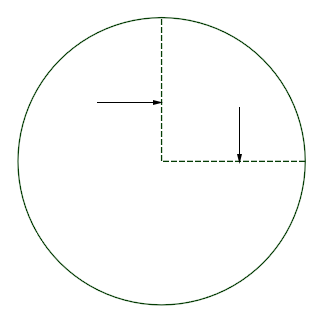
\includegraphics[width=\textwidth]{images/periodic/rotper2.png}
    \caption{ Rotational periodicity}
    \label{fig:rotper}
    \end{subfigure}
    \begin{subfigure}{0.69\textwidth}
    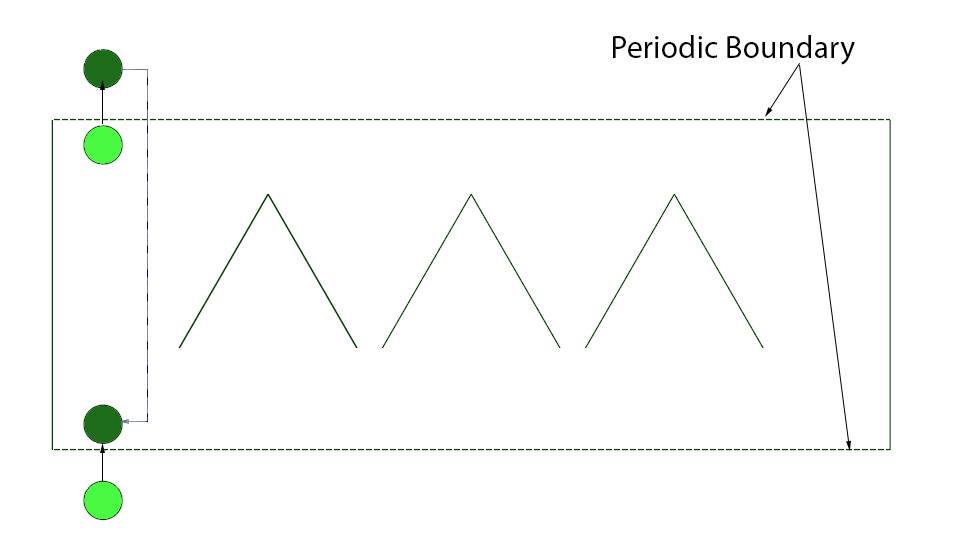
\includegraphics[width=\textwidth]{images/periodic/periodic2.png}
    \caption{ Translational periodicity }
    \label{fig:traper}
  \end{subfigure}
  \caption{Depiction of the periodic boundary}
\end{figure}

\noindent Periodic boundaries are of two kinds: Rotational and Translational. Rotational periodic boundaries usually subtend an angle about a rotationally symmetric body's centre line as can be seen in figure \ref{fig:rotper}.

On the other hand, translationally periodic boundaries form periodic planes in linear geometry, as can be seen in figure \ref{fig:traper} (Inspired by \cite{fluth} and \href{https://en.wikipedia.org/wiki/Periodic_boundary_conditions#/media/File:Limiteperiodicite.svg}{Grimlock, Wikimedia commons}).



% Equation~\ref{eq.1} is an example on how to add simple equation:

% \begin{equation}
% p_{1} +\frac{1}{2}\rho v_{1}^{2} +\rho g h_{1}=p_{2}+\frac{1}{2}\rho v_{2}^{2}+\rho g h_{2}+\Delta p_{f}+\rho w_{t} 
% \label{eq.1}																			
% \end{equation}

% \vspace{1cm}

% \noindent
% Equation~\ref{eq.2} is an example on how to add a large equation:

% \begin{equation}
% 	\lambda = \left\{ 
% 	   \begin{array}{l l}
%      \frac{64}{Re} & \quad 	\ Re < 2300 \\ \\
%      \frac{0.316}{\root 4\of{Re}} &\quad 	\ 2300 < Re < 10^{5} \\
% 	   \end{array} \right.
% 	\label{eq.2}													
% \end{equation}

% \subsubsection{Heading level 3}

% \vspace{.3cm}

% \noindent
% Body text $...$

% \subsubsection*{Heading level 4}

% \vspace{.3cm}

% \noindent
% Body text $...$

%%%%%%%%%%%%%%%%%%%%%%%%%%%%%%%%  Chapter 3  %%%%%%%%%%%%%%%%%%%%%%%%%%%%%%%%%%%%%%%%%%%
\clearpage
\thispagestyle{empty}

\cleardoublepage

\thispagestyle{plain}

\section{Method}\label{sec:method}
\vspace{.6cm}
This section presents the methodology that was followed to conduct the study. The experimental setup, and conditions are given, followed by the workflow for the CFD study, including the generation of the model, the mesh, mesh insensitivity study and the setup of the Fluent solver.

\subsection{Experimental Setup}
\vspace{0.3cm}
In order to obtain the experimental results, the heat pump was placed in a climate chamber, at  $101325\ Pa,\ 275\ K$. Pressure sensors were placed between the evaporator and fan, and after the evaporator in order to measure the pressure drop caused by the evaporator(as can be seen in figure \ref{fig:pnid}).
\begin{figure}[!ht]
    \centering
    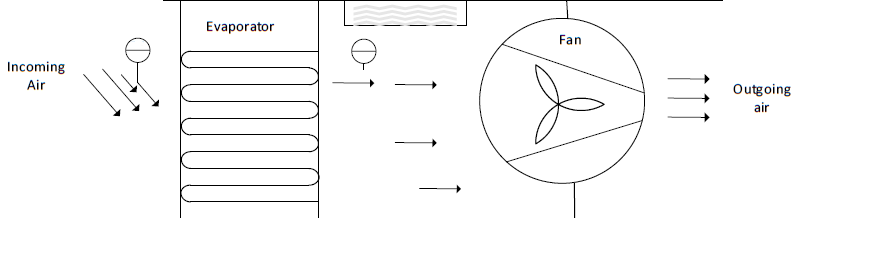
\includegraphics[width=0.8\textwidth]{images/pnID2.png}
    \caption{Experimental Setup}
    \label{fig:pnid}
\end{figure}
Refrigerant from the compressor was inlet into the evaporator at a pressure of $300\ kPa$ with a mass flow of $0.252\ kg/s$. From the evaporator data sheet, it is known that the evaporating temperature is $-3 \degree C/270\ K$. After letting the device run, the pressure difference is calculated, and the equations in section \ref{app:presd} is used to estimate the ice thickness. The calculated ice thickness after performing the experiment can be seen in figure \ref{fig:expchart} below:
\begin{figure}[!ht]
    \centering
    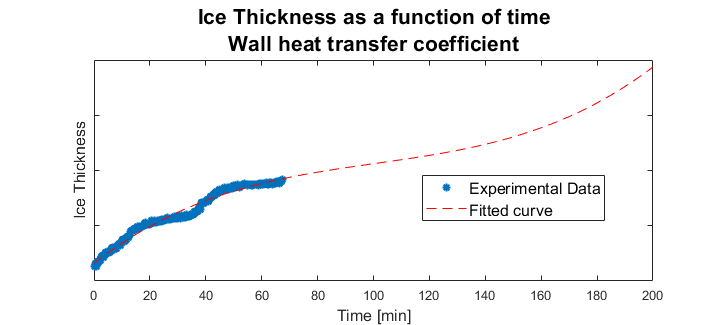
\includegraphics[width=0.8\textwidth]{images/expchart2.png}
    \caption{Chart of experimental (calculated) ice thickness as a function of time}
    \label{fig:expchart}
\end{figure}

\subsubsection{Pressure Difference to Ice Thickness Relations}\label{app:presd}
\vspace{.3cm}
While performing the experimental study, it is not possible to directly calculate the thickness of the ice built up on the evaporator. Thus, this needs to be calculated empirically from results already obtained by Bosch. %This empirical relation is seen in equation \ref{eq:delpice} below. The relation used in order to calculate the pressure drop from the ice thickness can be seen in equation \ref{eq:icedelp}:
% \begin{align}
%     \label{eq:delpice}
%     z&=4.9694\Delta P^2+6.6542\Delta P+11.705\\
%     \label{eq:icedelp}
%     \Delta P&=-0.00196z^2+0.15471z-1.52788
% \end{align}
In the CFD simulation, the obtained ice thickness was used to calculate the pressure drop (section \ref{sec:method}). Empirical relations were further used (as provided by Bosch) in order to calculate the velocity based on the properties of the fan. These equations are shown as equation \ref{eq:fancurve} below.
\begin{align}
    \label{eq:fancurve}
    \begin{split}
        \lambda&=\frac{\Delta P/\rho}{N^2 D^2}\\
        \Phi&=f(\lambda)\\%-40.4\lambda^2-1.097\lambda+0.1314\\
        V&=N D^2 \phi\\
        u&=V/A
    \end{split}
\end{align}
Where $\lambda$ is the head coefficient, $N$ is the speed of the fan (in rad/s), $D$ is the fan diameter (in m), $\phi$ is a factor that relates the flow head to the flow rate, $V$ is the volume flow rate over the evaporator ($m^3/s$) and $A$ is the area of the evaporator that is facing the air-flow (in $m^2$). The velocity as predicted by this set of equations can be seen in figure \ref{fig:projvel} below:
\begin{figure}[!ht]
    \centering
    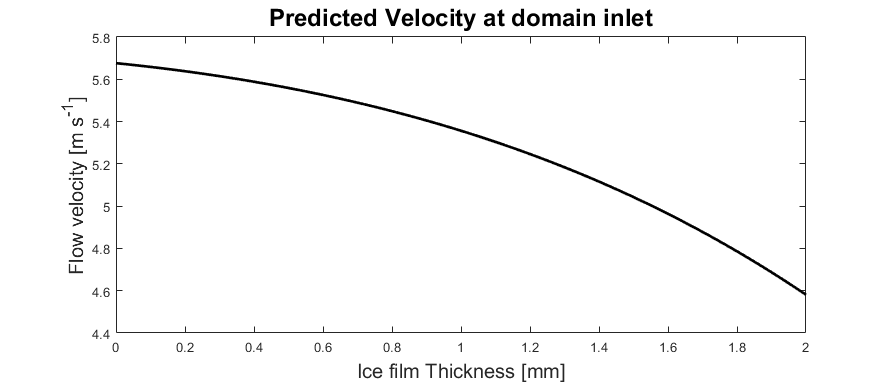
\includegraphics[width=\textwidth]{images/projvel.png}
    \caption{Velocity prediction based on equation \ref{eq:fancurve}}
    \label{fig:projvel}
\end{figure}

\subsection{CAD model}
\vspace{0.3cm}
A CAD model of the evaporator was provided by the company including walls and pipes. The provided NX file was imported into Ansys SpaceClaim, and the  provided model can be seen in figure \ref{fig:originalmodel}. In order to reduce the complexity of the geometry prior to simulation, bolt holes and side walls were removed, and fins were added to the model. Additionally, the pipes were ensured to be connected without gaps.
Figure \ref{fig:fullevap} shows the top view of the evaporator after said cleaning. Figure \ref{fig:pipecirc} shows the piping circuit diagram for the evaporator provided by the manufacturer.
\begin{figure}[!ht]
    \centering
    \begin{subfigure}{0.8\textwidth}
    \centering
    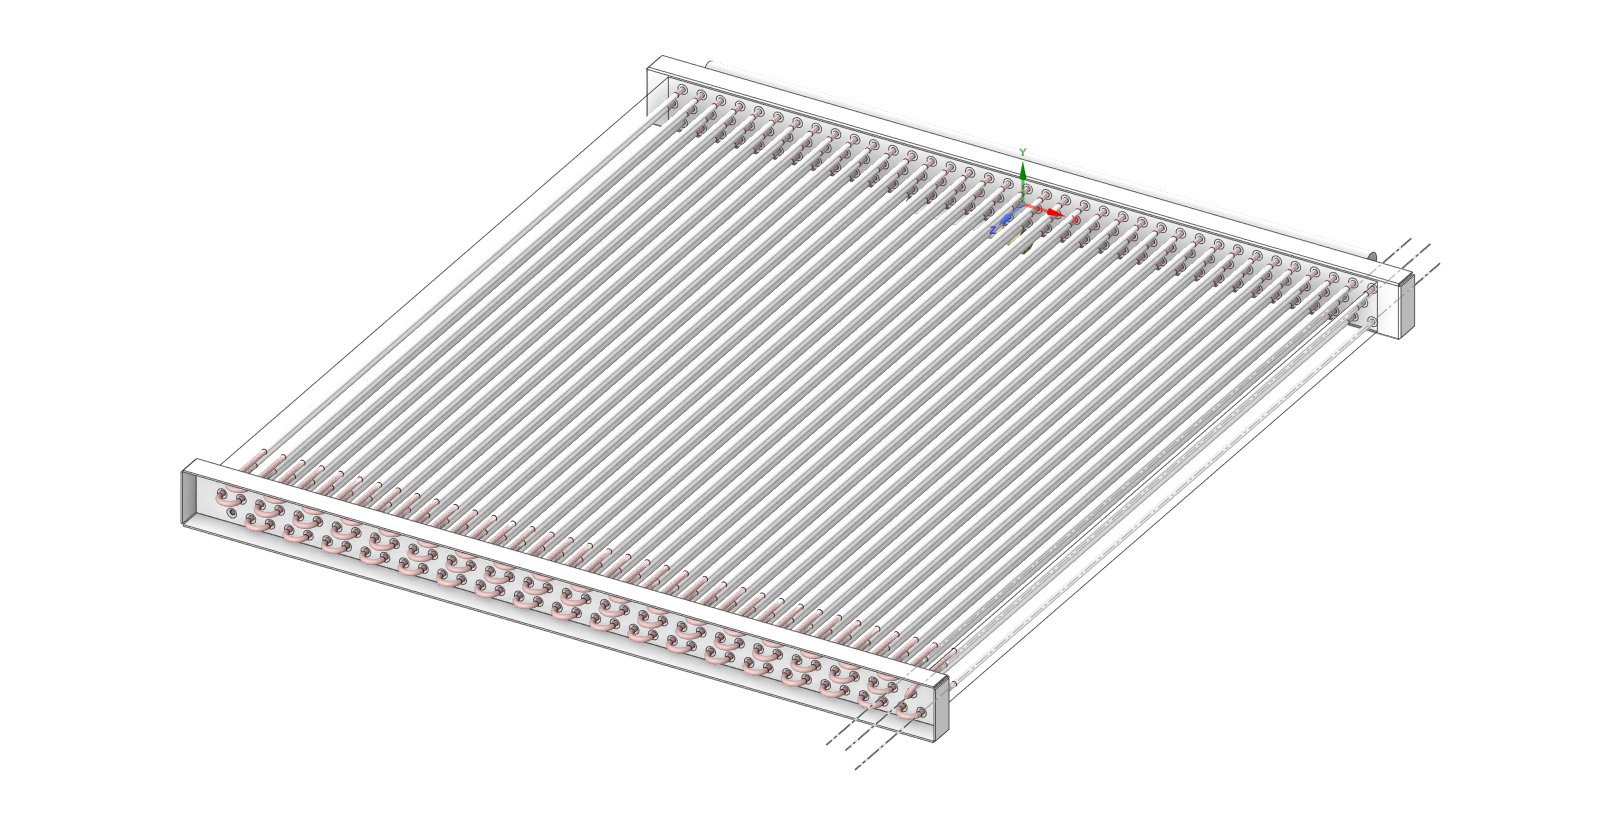
\includegraphics[width=\textwidth]{images/evaporator_provided.png}
    \caption{Provided original CAD model}
    \label{fig:originalmodel}
    \end{subfigure}
    \begin{subfigure}{0.8\textwidth}
    \centering
    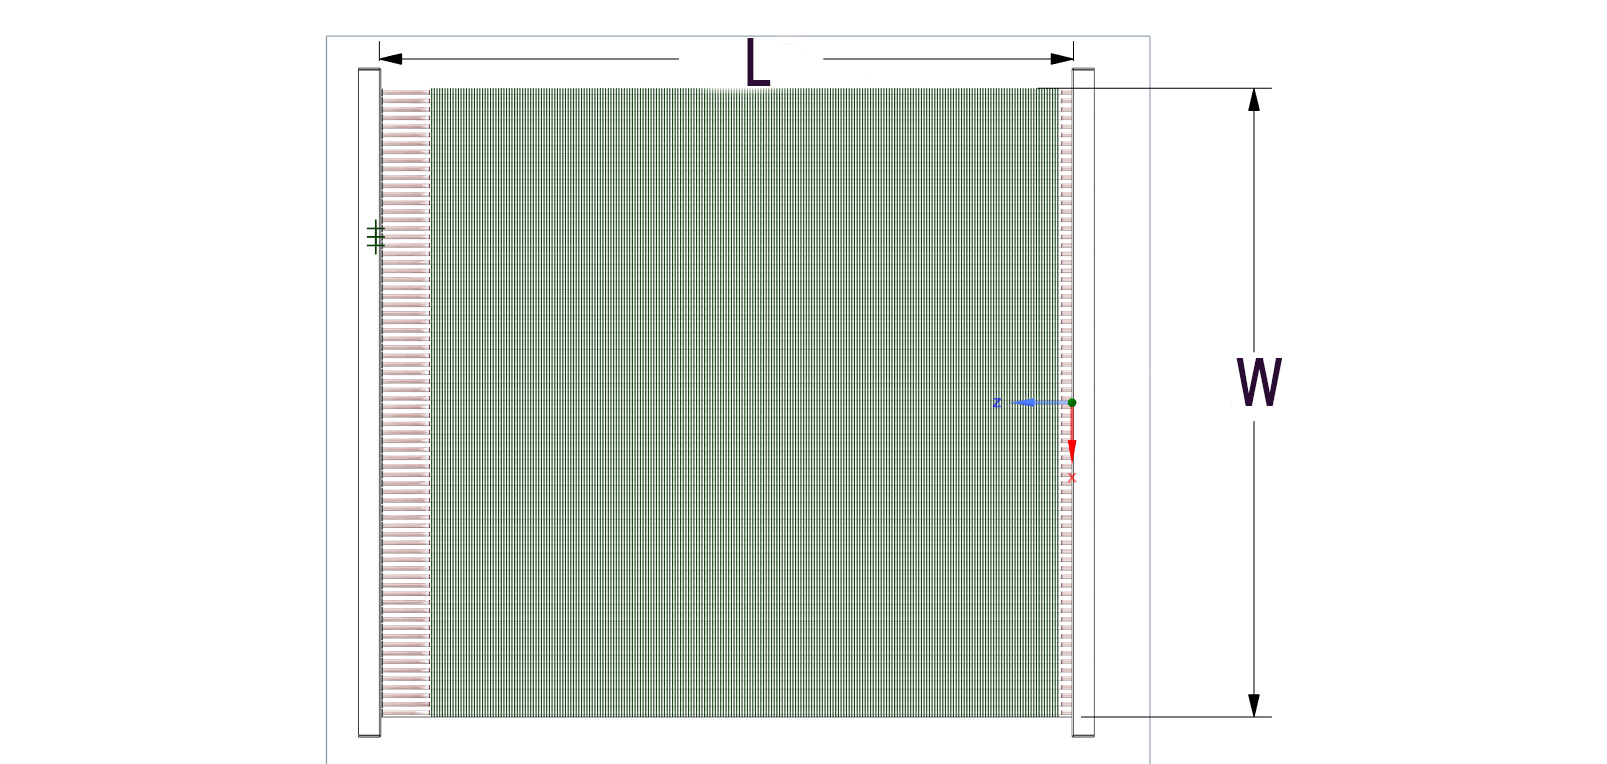
\includegraphics[width=\textwidth]{images/geomfull.png}
    \caption{Full evaporator - top view (with the fins shown in gren)}
    \label{fig:fullevap}
    \end{subfigure}
    \caption{Full size evaporator model}
    \label{fig:originalfullevap}
\end{figure}
\begin{figure}[!ht]
    \centering
    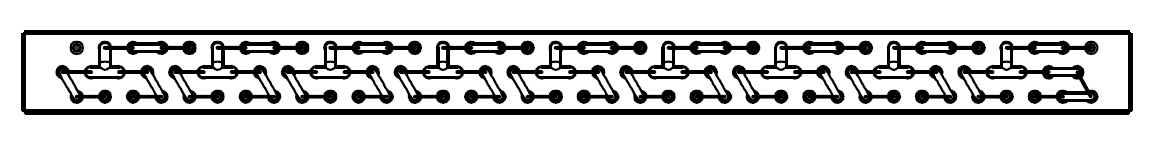
\includegraphics[width=\textwidth,trim=0 0 0 0,clip]{images/pipecirc.png}
    \caption{Piping circuit and connections}
    \label{fig:pipecirc}
\end{figure}
\pagebreak
\subsubsection{Simplified Geometry}
\vspace{0.3cm}
{In order to reduce the simulation and meshing time}, a scaled down CAD model of the evaporator was generated in Ansys SpaceClaim. The sizing was arbitrarily chosen to include 3 rows of pipes as can be seen in figure \ref{fig:simplegeom}. Only 5 (identical) fins were included, and the fin spacing was maintained as in the full scale evaporator ($3.00mm$). This is to ensure the physics of the simulations worked as expected and debug any potential errors. As can be seen in figure \ref{fig:simplgeomiso}, the gray shaded faces (and the faces opposite to them) are the walls of the evaporator, the blue face is the air inlet and the pink face (and the opposite face) are the periodic boundaries. These are a translationally periodic boundary pair (see section \ref{sec:periodicbc}). Figure \ref{fig:outergeom} shows the simplified geometry compared to the original evaporator wall.

\begin{figure}[!ht]
    \centering
    \begin{subfigure}{0.49\textwidth}
    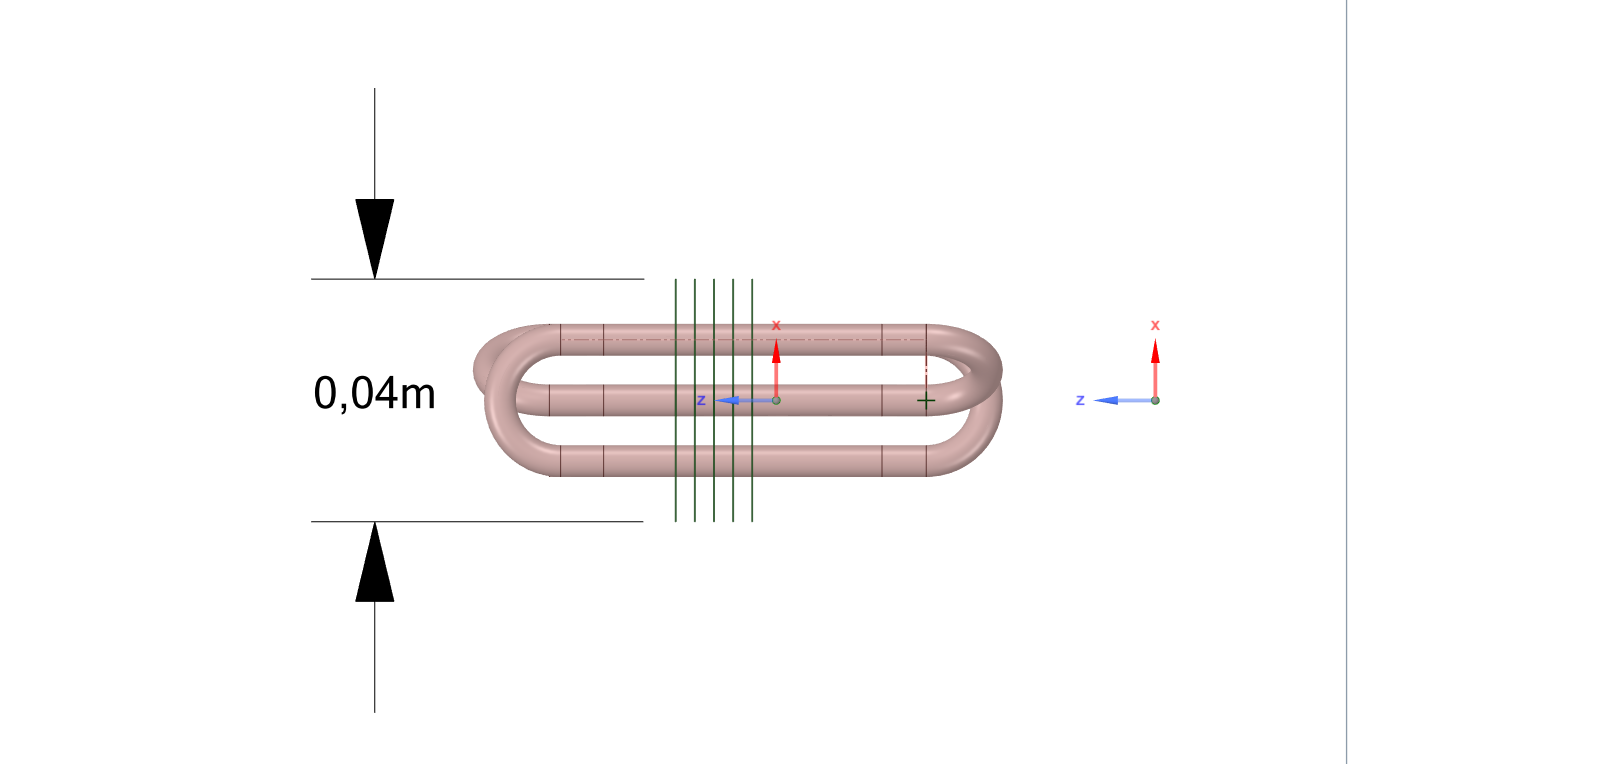
\includegraphics[width=\textwidth,trim=10 10 200 10,clip]{images/geomcut_top.png}
    \caption{Top View} 
    \label{fig:cuttop}
    \end{subfigure}
    \begin{subfigure}{0.49\textwidth}
    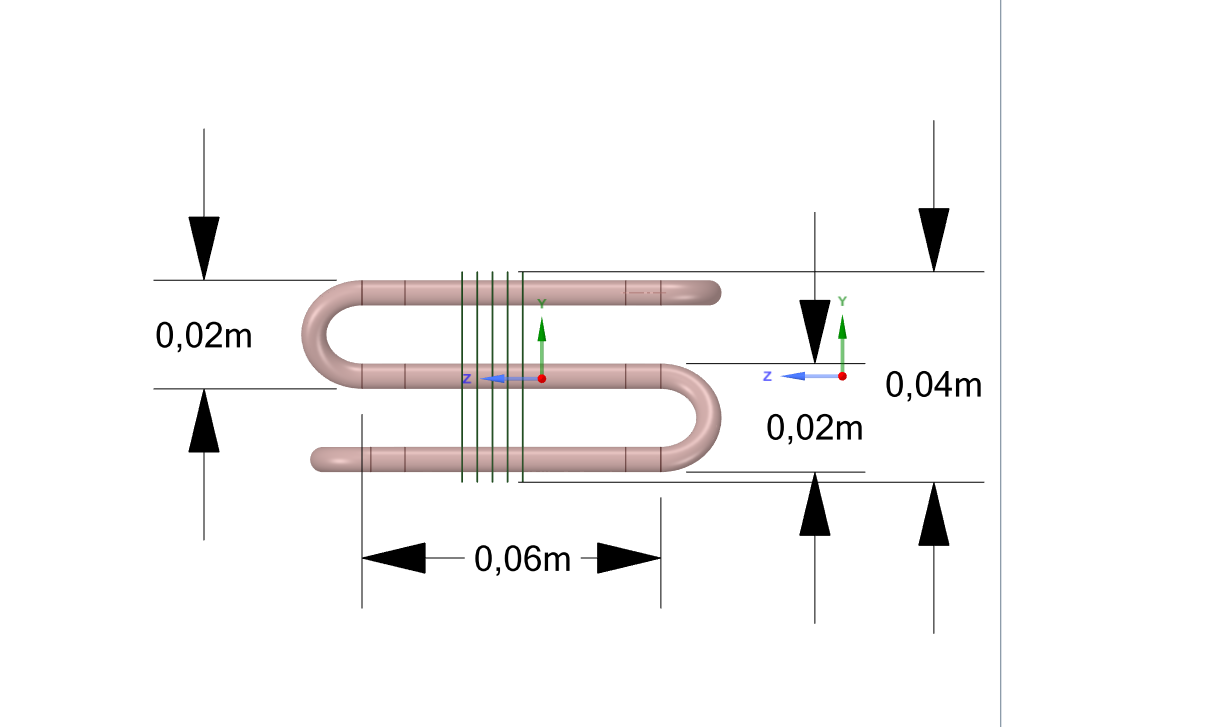
\includegraphics[width=\textwidth,trim=10 10 100 10,clip]{images/geomcut_side.png}
    \caption{Side View}
    \label{fig:cutside}
    \end{subfigure}
    % \begin{subfigure}{0.49\textwidth}
    % 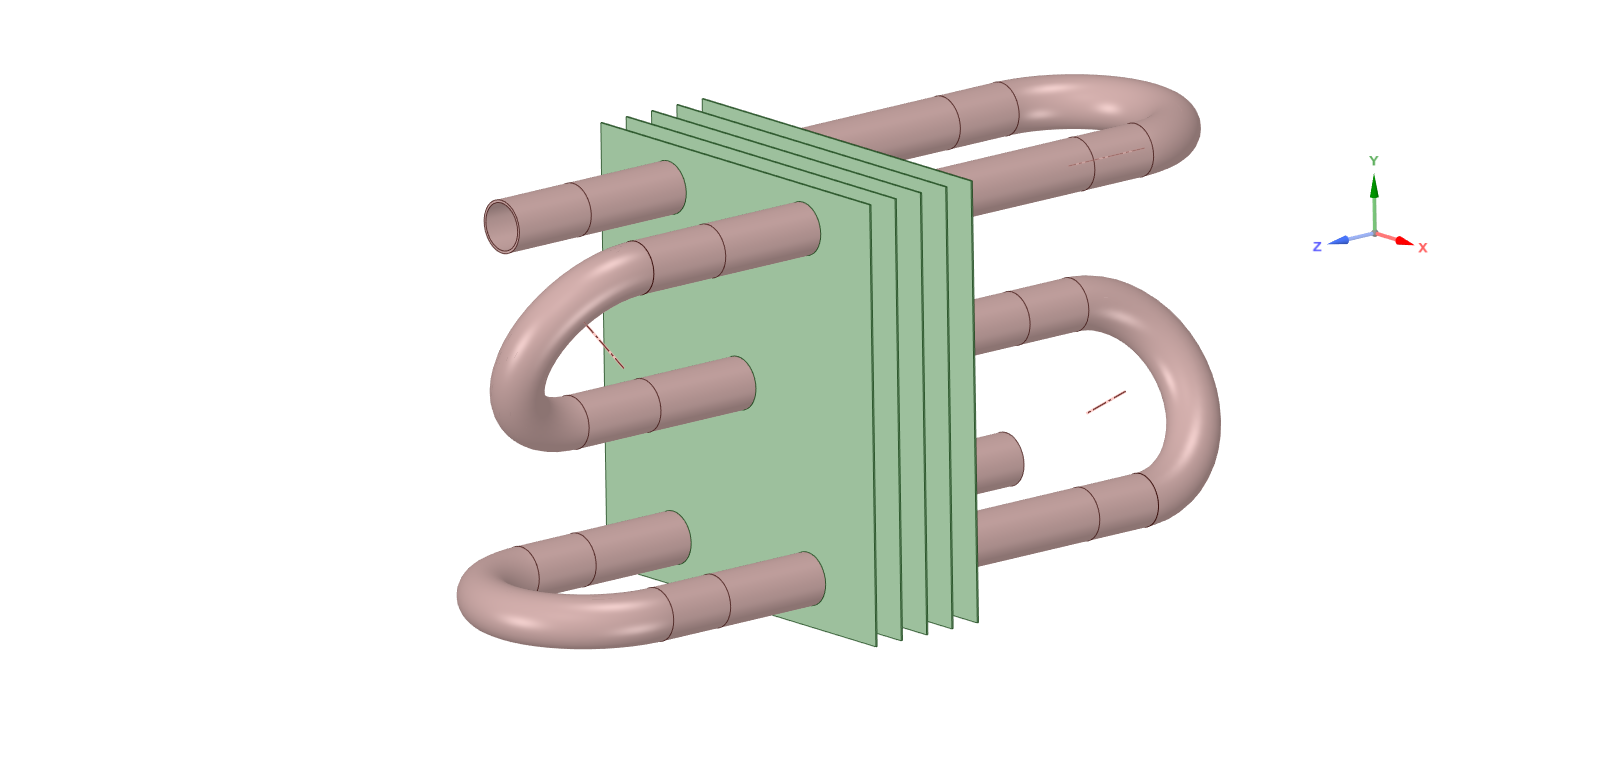
\includegraphics[width=\textwidth,trim=10 10 100 10,clip]{images/Geom-3.png}
    % \caption{Iso View}
    % \label{fig:cutiso}
    % \end{subfigure}
    \caption{Simplified Geometry of evaporator}
    \label{fig:simplegeom}
\end{figure}
\begin{figure}[!ht]
    \centering
   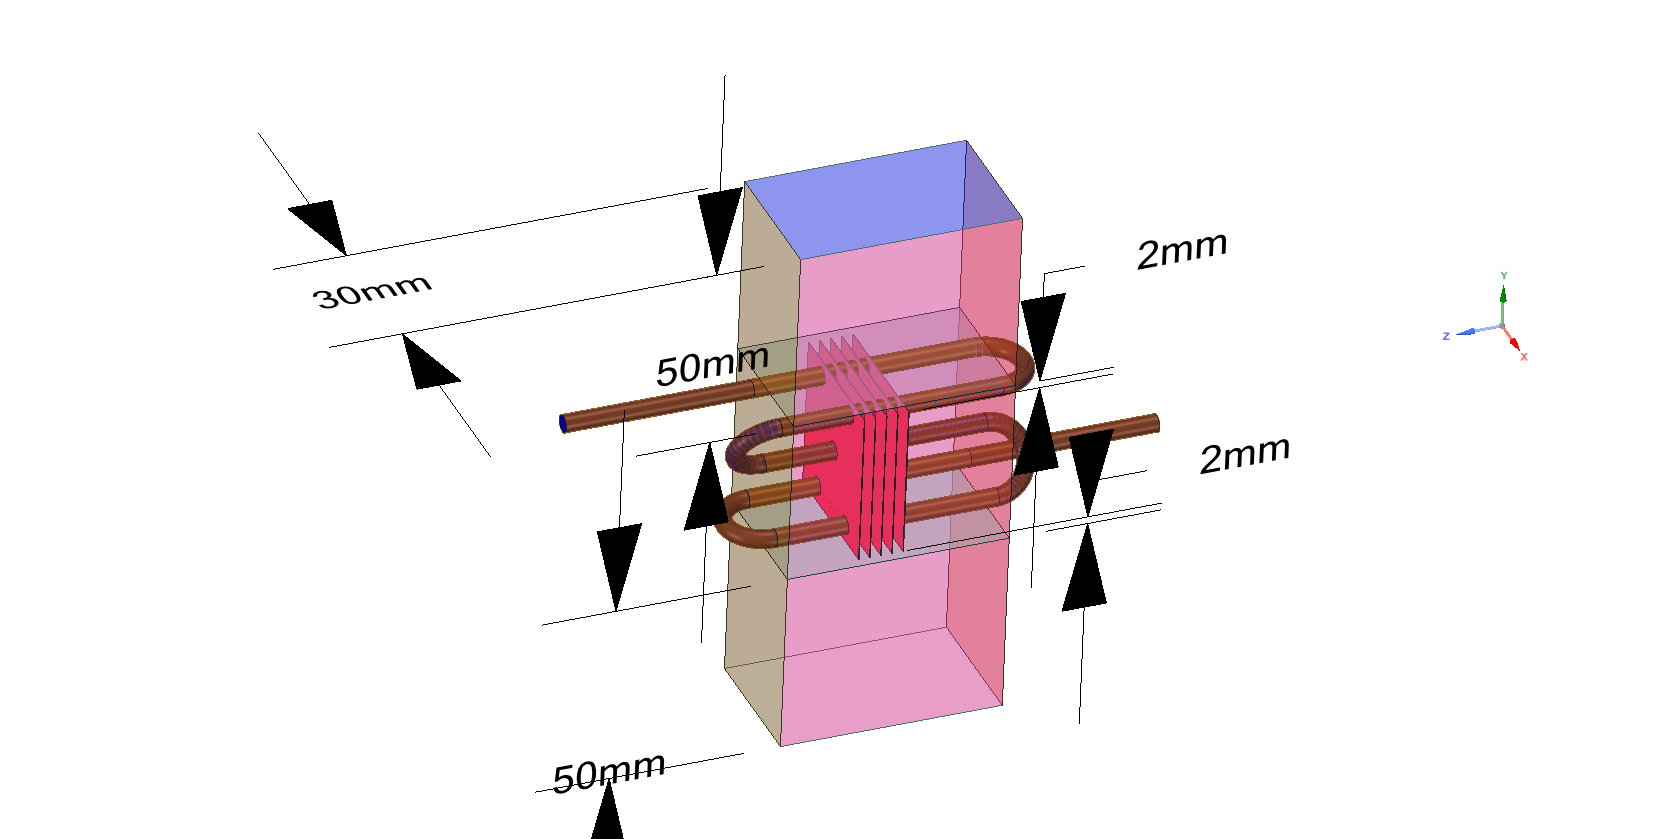
\includegraphics[width=0.8\textwidth,trim=4cm 0 4cm 0,clip]{images/geom_up/planned_scale.png}
   \label{fig:sidemeasure}
   \caption{Isometric View with domain}
   \label{fig:simplgeomiso}
\end{figure}
\begin{figure}[!ht]
    \centering
    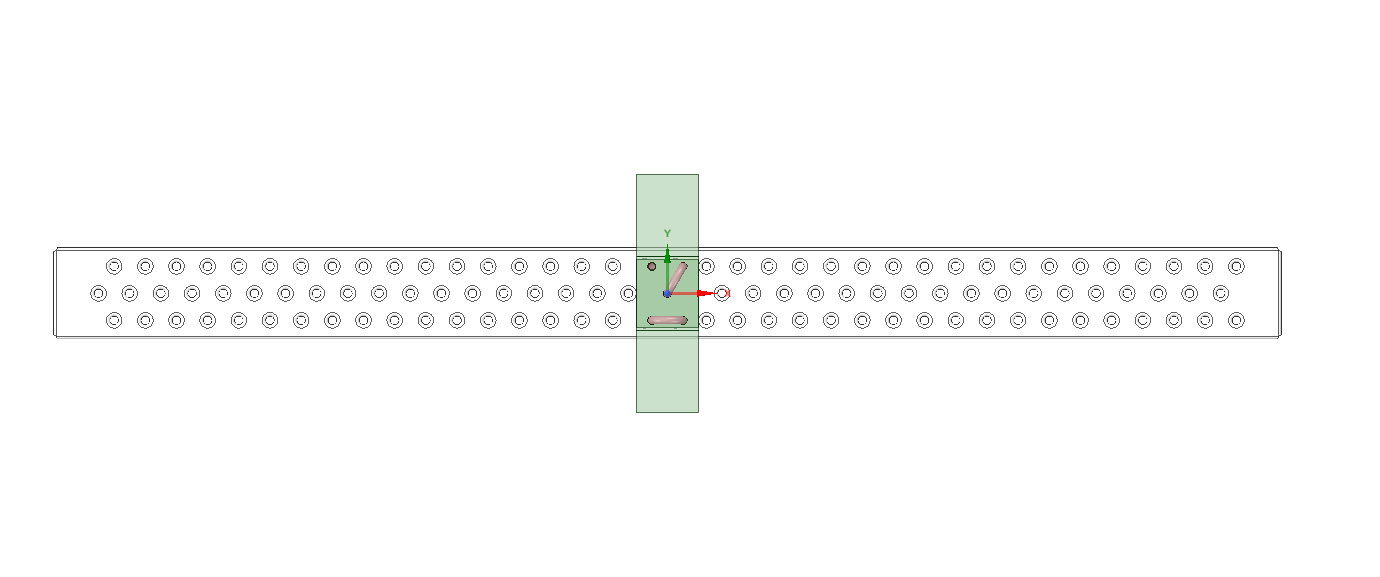
\includegraphics[width=0.8\textwidth]{images/comparer.PNG}
    \caption{Simplified geometry with domain, shown with original evaporator walls to scale}
    \label{fig:outergeom}
\end{figure}
\begin{figure}[!ht]
    \centering
    \begin{subfigure}{0.49\textwidth}
    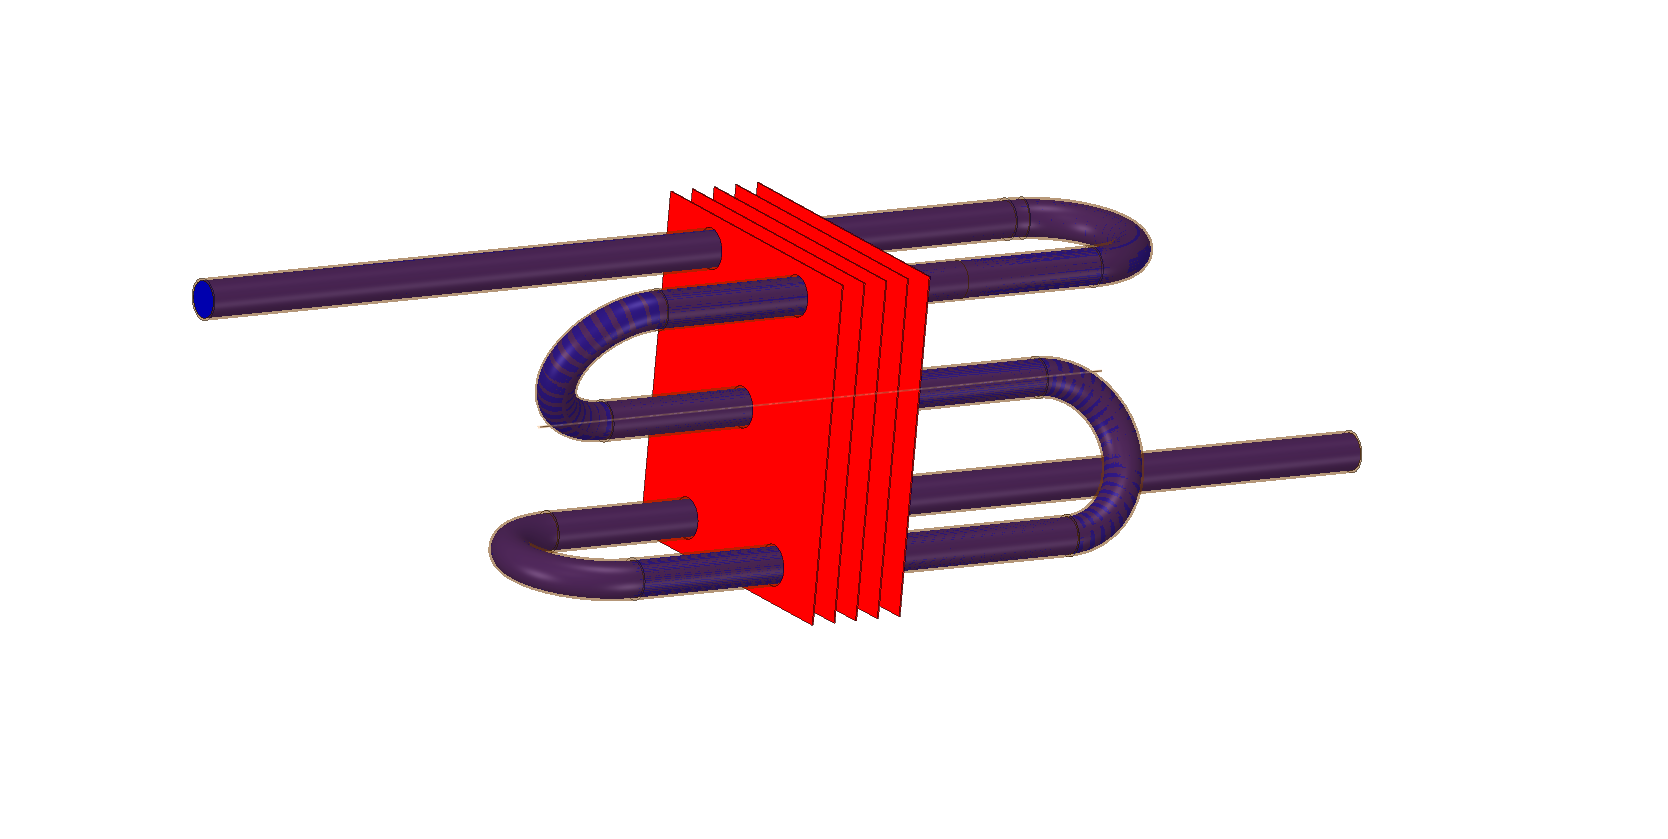
\includegraphics[width=\textwidth,trim=10 10 200 10,clip]{images/geom_up/internal flow.png}
    \caption{Internal Flow domain}
    \label{fig:newint}
    \end{subfigure}
    \begin{subfigure}{0.49\textwidth}
    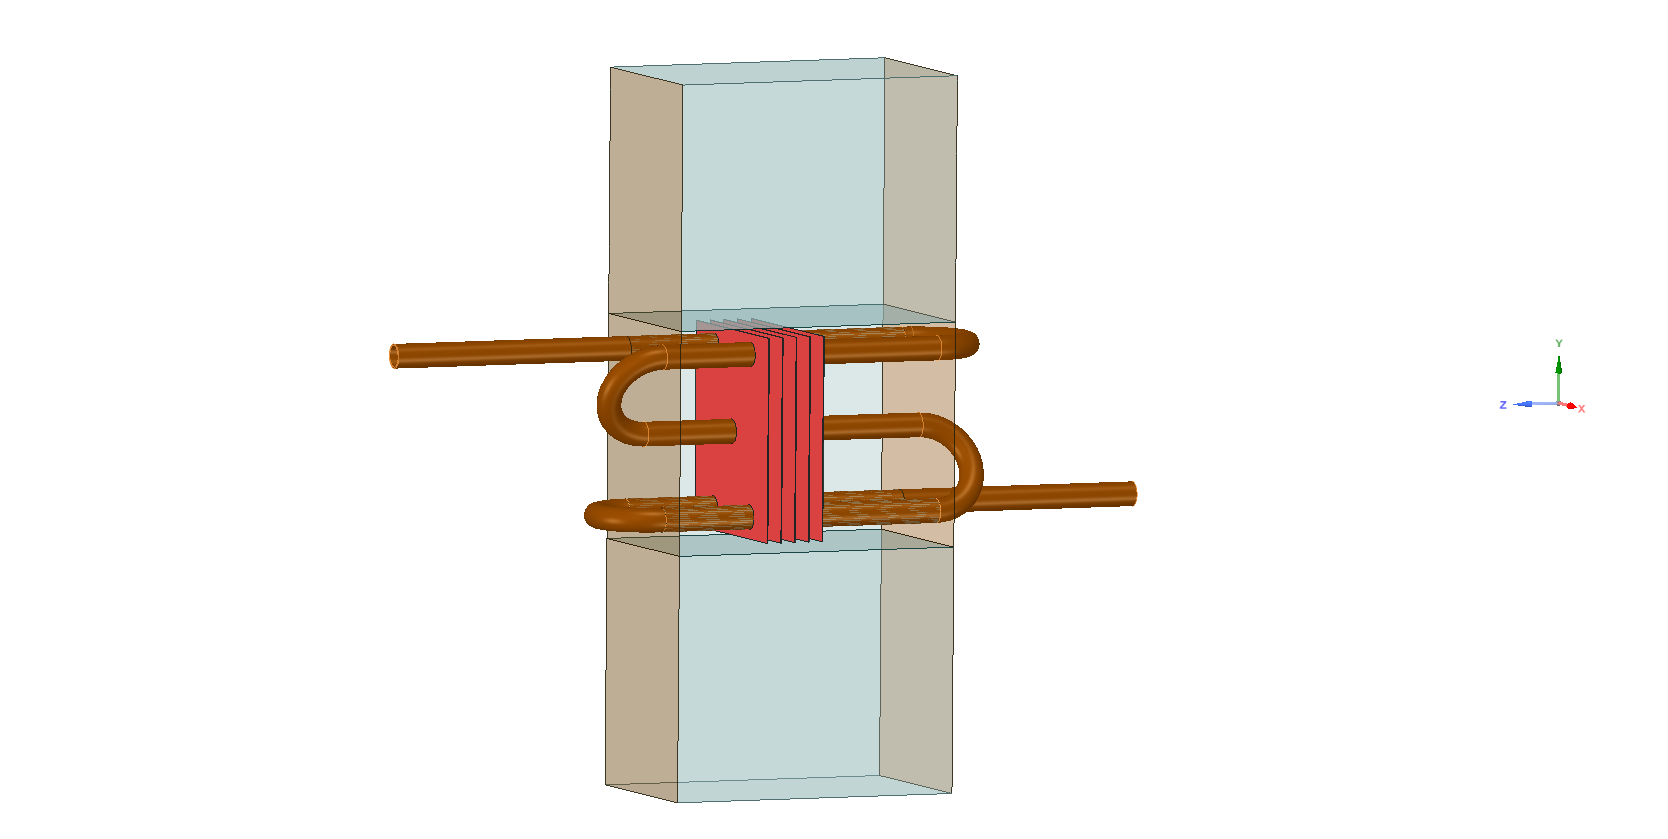
\includegraphics[width=\textwidth,trim=10 10 100 10,clip]{images/geom_up/external_flow.png}
    \caption{External Flow domain}
    \label{fig:newext}
    \end{subfigure}
    \caption{Separated Flow domains}
    \label{fig:newnewnew}
\end{figure}

\begin{figure}[!ht]
    \centering
    \begin{subfigure}{0.49\textwidth}
    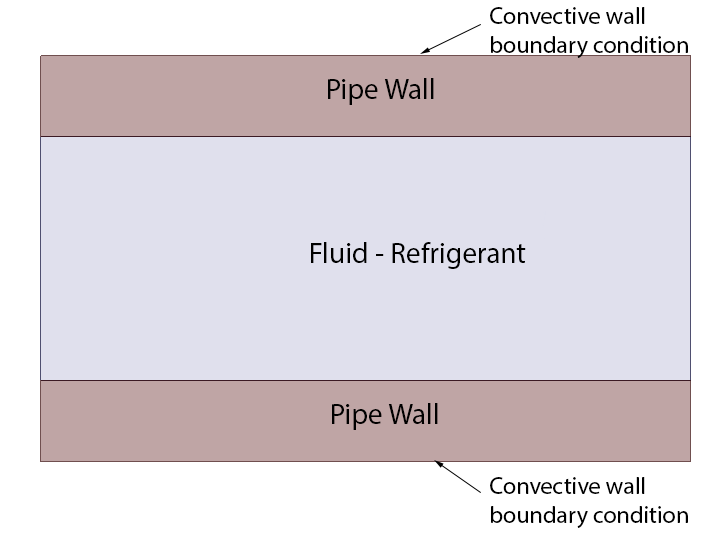
\includegraphics[width=\textwidth]{images/geom_up/pipebc1.png}
    \caption{Internal Flow domain}
    \label{fig:new2int}
    \end{subfigure}
    \begin{subfigure}{0.49\textwidth}
    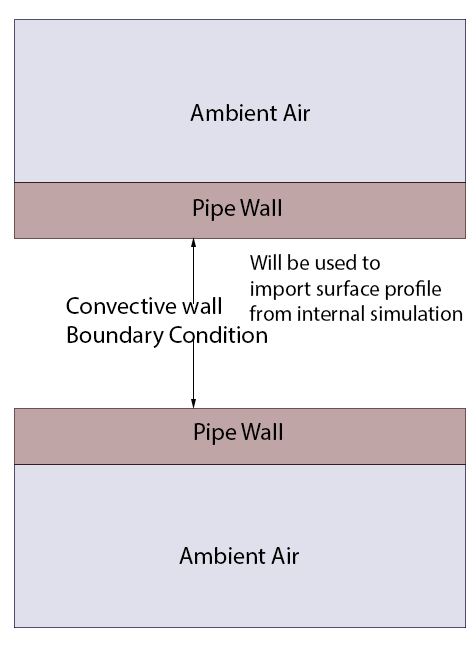
\includegraphics[width=\textwidth]{images/geom_up/pipebc1_e.png}
    \caption{External Flow domain}
    \label{fig:new2ext}
    \end{subfigure}
    \caption{Block diagram showing pipe and boundary condition}
    \label{fig:new2}
\end{figure}

% \begin{figure}[!ht]
%     \centering
%     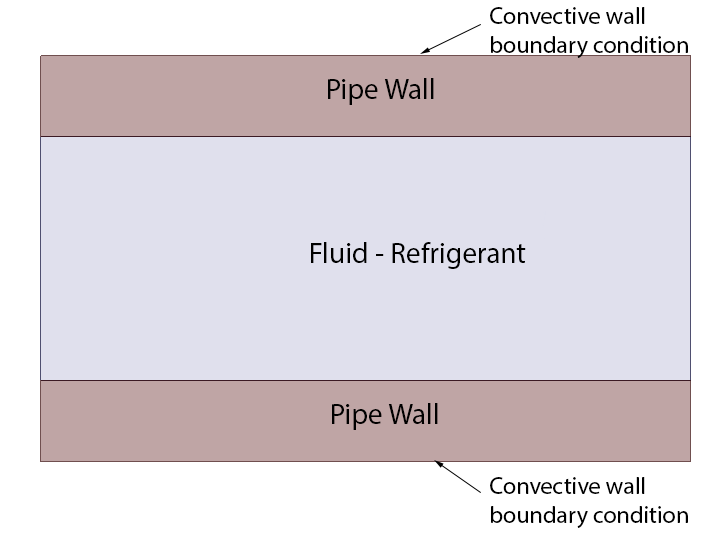
\includegraphics[width=0.49\textwidth]{images/geom_up/pipebc1.png}
%     \caption{Block diagram showing pipe and boundary condition  - Internal Flow domain}
%     \label{fig:new2int}
% \end{figure}
% \begin{figure}[!ht]
%     \centering
%     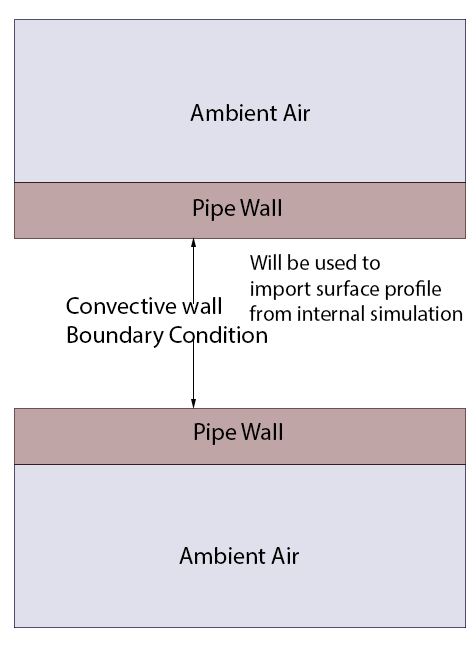
\includegraphics[width=0.49\textwidth]{images/geom_up/pipebc1_e.png}
%     \caption{Block diagram showing pipe and boundary condition - External Flow domain}
%     \label{fig:new2ext}
% \end{figure}
Due to the presence of two different fluids undergoing phase change and the limitations of current CFD software, it was not possible to perform the entire study within one simulation. Thus, it was necessary to split the internal and external flows for the evaporator. The internal flow simulation would include the phase change of the refrigerant, whereas the external flow would include phase change of water vapour. This split was done such that the solid surfaces of the evaporator and pipes would be common to both the simulations (as explained in section \ref{sec:extflowsts}). Figures \ref{fig:newint} and \ref{fig:newext} show the domains for the internal and external simulations respectively. Within the internal flow geometry, the purple coloured region is showing the inner walls of the pipe. Figures \ref{fig:new2ext} and \ref{fig:new2int} show a block diagram of the pipe. For the internal flow simulation, the outer wall is set to a constant convective boundary condition (explained in section \ref{sec:internalsolv}). Within the external flow domain, the temperature and heat transfer coefficient from the internal flow simulation would be imported as surface profiles (See section \ref{sec:externalsolv}).

\subsection{Physics Options}
\vspace{0.3cm}
For the external flow, icing will be simulated as a phase change and deposition of water vapour from air. For the internal flow, evaporation of the propane refrigerant will be simulated, taking heat from the surroundings. Heat transfer between the flows will be linked using 'Surface Profiles'. According to the Fluent User's Guide \cite{flug}, it is used to define the boundary conditions for one flow based on the results of another simulation. Section \ref{sec:extflowsts} explains this in more detail.\\
In terms of the materials, the fins were simulated as aluminium bodies while the pipes were copper. The refrigerant was simulated using multi-phase propane (both liquid and vapour phases were defined, as defined in Appendix \ref{app:code}.



\subsection{Mesh Generation}
\vspace{0.3cm}
Separate meshes were generated for the internal and external flows. Both situations required heat transfer through solids, and thus the solid walls were meshed as well. Both the meshes were generated using the watertight workflow in Fluent. This workflow method is a guided procedure available in Ansys Fluent that allows the generation of a mesh in a step-by-step process without the need for a script, while also providing full control over all the parameters. The additional advantage was the enable ease of transfer of work for Bosch internally, since this was the method already in use by the company.

\subsubsection{External Flow}
\vspace{0.3cm}
For the case of the external flow, a minimum surface element size of $2.04\times 10^{-4}\ m$ and a maximum element size of $3.02\times 10^{-3}\ m$ were used, with a growth rate of 1.2. Additionally, the scoping proximity was set to faces so as to enable exponential growth (supporting boundary layers) at the intersection of two faces. The opposite ends of the fins and the side walls were subsequently set to be translationally periodic (In order to imitate a larger domain while maintaining a small domain, as detailed in section \ref{sec:periodicbc}). While the geometry was generated, there were overlapping faces present at the intersection of the fluid and solid regions of the model. In order to eliminate these, an `Apply Share Topology' task was added with the default gap size marked. This would ensure that the overlapping faces would be merged automatically. After the fluid region was defined (one region, air), boundary layers were defined on the surfaces of the pipes and the fins. Five layers of inflation were set to grow on the walls with a the 'smooth transition' setting and a growth rate of $1.2$. From previous studies conducted by the company, this number was deemed to provide the necessary accuracy to the solution, while not being computationally heavy. Additionally, the obtained average y+ was $~35$, in which case Fluent uses the `Automatic Wall Function' that reduces the sensitivity to the near-wall mesh size\cite{flug}. Finally, an `Improve Volume Mesh' task was added. This operation reduces cell skewness by automatically collapsing cells as needed. The generated mesh can be seen in figure \ref{fig:meshext}.

\begin{figure}[!ht]
    \centering
    \begin{subfigure}{0.49\textwidth}
    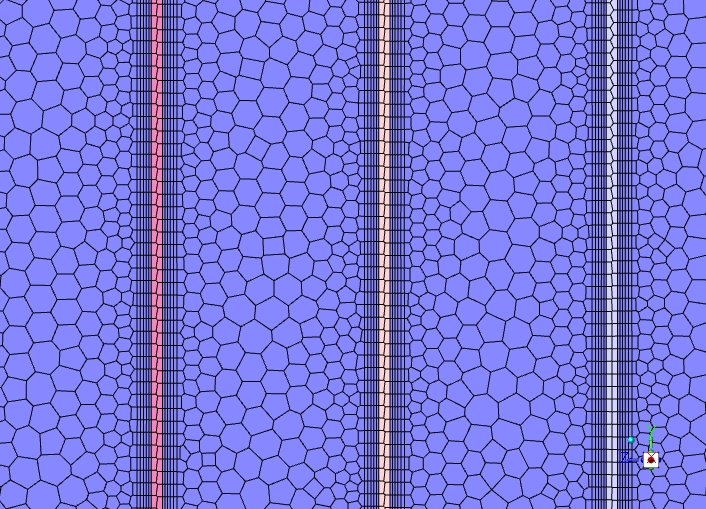
\includegraphics[width=0.95\textwidth]{images/mesh_fin.jpg}
    \caption{Close-up view of fins}
    \end{subfigure}
    \begin{subfigure}{0.49\textwidth}
    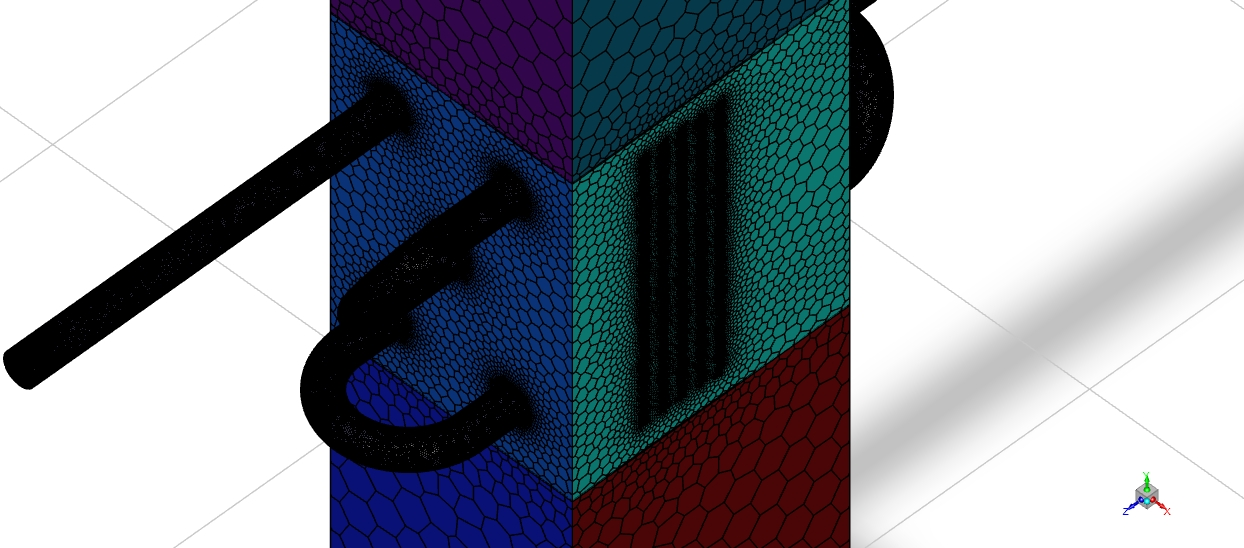
\includegraphics[width=0.95\textwidth]{images/external_full.jpg}
    \caption{Isometric View}
    \end{subfigure}
    \caption{Generated mesh for the external flow simulation}
    \label{fig:meshext}
\end{figure}

\subsubsection{Internal Flow}\label{sec:meshint}
\vspace{0.3cm}
For the internal flow case, the minimum surface element sizes (across all the faces of the model) were the same as in the external flow case. This was done so the walls have the same number of nodes and the surface profiles can be linked in a straightforward way. The only difference was the number and size of the boundary layers. 10 inflation layers with a smooth transition were used with a ratio of 0.272 for the fluid. The 'Poly-hexcore' meshing method was selected, as this would enable multi-threaded meshing and drastically {increase} the speed\cite{ansyspolyhex}. The additional benefit of using this method is that there is a good blend between the coarse and fine mesh regions. Finally, an 'Improve Volume Mesh' task was added here as well, which improves the mosaic meshing quality. The internal flow generated mesh can be seen in figures \ref{fig:meshint} and \ref{fig:meshint2}. 

\begin{figure}[!ht]
    \centering
    \begin{subfigure}{0.49\textwidth}
    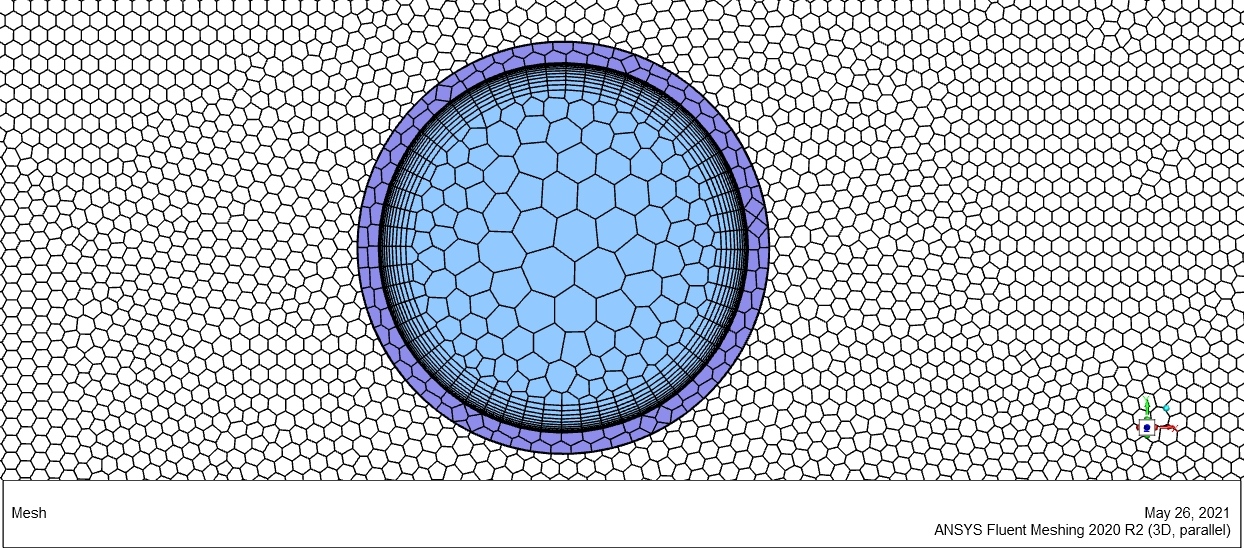
\includegraphics[width=0.8\textwidth]{images/internal_pipe_mesh.jpg}
    \caption{Front view}
    \label{fig:meshint}
    \end{subfigure}
\begin{subfigure}{0.49\textwidth}
    \centering
    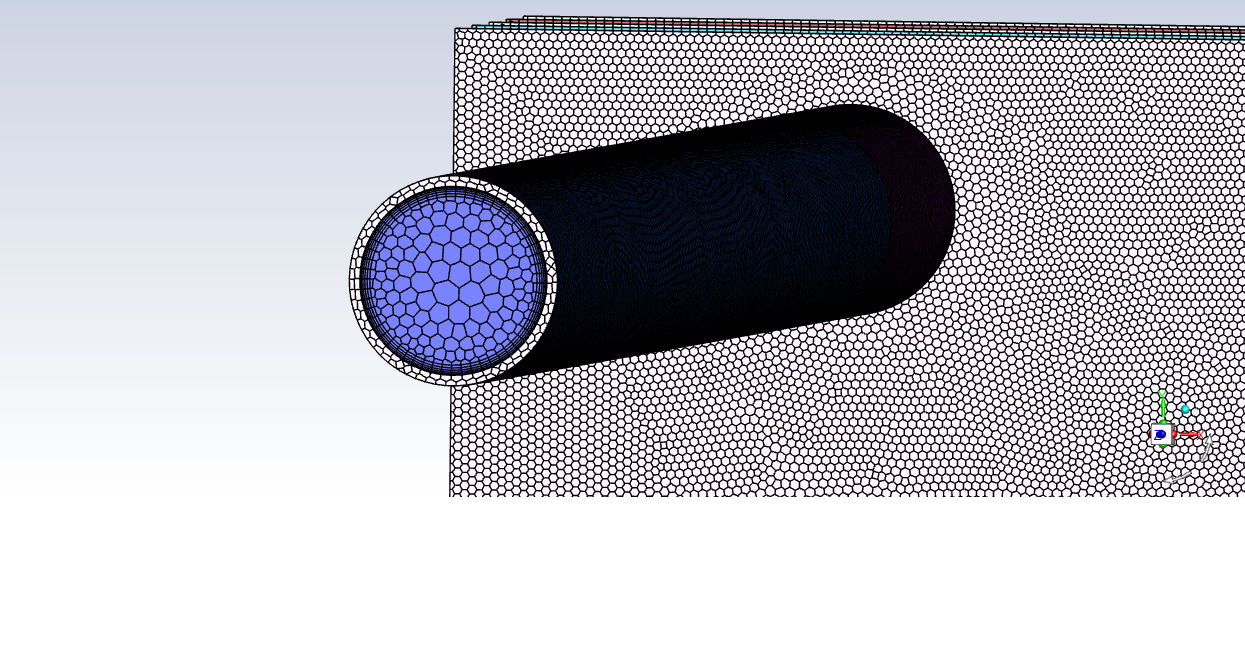
\includegraphics[width=0.8\textwidth]{images/pipe_mesh.png}
    \caption{Perspective View}
    \label{fig:meshint2}
\end{subfigure}
\caption{Mesh used for internal flow simulation, zoomed in on pipe to show boundary layers. Fin in background}
\end{figure}



\subsection{Mesh Sensitivity Study}
\vspace{0.3cm}
In order to ensure that the results were independent of the mesh size used, a sensitivity analysis was conducted on the impact of the number of elements and the precision of the results. The results of this study can be seen in tables \ref{tab:meshsens_out} and \ref{tab:meshsens_in} below. Additionally, the relevant figures of the plots can be seen in figures \ref{fig:meshsens_out} and \ref{fig:meshsens_in}.\\

% Please add the following required packages to your document preamble:
% \usepackage{graphicx}
\setcounter{table}{0}
\begin{table}[!ht]
\centering
\caption{Mesh Sensitivity data for external flow}
\label{tab:meshsens_out}
\resizebox{\textwidth}{!}{%
\begin{tabular}{|c|c|c|c|c|c|}
\hline
Mesh &
  \begin{tabular}[c]{@{}c@{}}Number of\\ elements (million)\end{tabular} &
  \begin{tabular}[c]{@{}c@{}}Average Pressure\\ Drop {[}Pa{]}\end{tabular} &
  \% Difference &
  \begin{tabular}[c]{@{}c@{}}Final ice film\\ thickness {[}mm{]}\end{tabular} &
  \% Difference \\ \hline
1 & 24.1 & 26.61 & 4.96 & 0.526 & 5.05 \\ \hline
2 & 44.5 & 28    & -    & 0.554 & -    \\ \hline
3 & 79.2 & 28.2  & 0.72 & 0.556 & 0.36 \\ \hline
\end{tabular}%
}
\end{table}
% \begin{table}[!ht]
% \centering
% \caption{Mesh Sensitivity data for external flow}
% \label{tab:meshsens_out}
% \begin{tabular}{|c|c|c|c|} 
% \hline
% Mesh & Number of elements (million) & Average Pressure Drop [Pa] & \% Difference  \\ 
% \hline\hline
% 1    &       24.1        &           26.61          &   4.96             \\ 
% \hline
% 2    &        44.5            &         28           & -              \\ 
% \hline
% 3    &         79.2           &          28.2         &   0.72             \\
% \hline
% \end{tabular}
% \end{table}

% Please add the following required packages to your document preamble:
% \usepackage{graphicx}
\begin{table}[!ht]
\centering
\caption{Mesh Sensitivity Data for internal flow}
\label{tab:meshsens_in}
\resizebox{\textwidth}{!}{%
\begin{tabular}{|c|c|c|c|c|c|}
\hline
Mesh &
  \begin{tabular}[c]{@{}c@{}}Number of \\ elements (million)\end{tabular} &
  \begin{tabular}[c]{@{}c@{}}Area wt avg of\\ Volume Fraction {[}-{]}\end{tabular} &
  \% Difference &
  \begin{tabular}[c]{@{}c@{}}Area wt avg of\\ Wall HTC {[}$W/m^2${]}\end{tabular} &
  \% Difference \\ \hline
1 & 16.05   & 0.9983 & - & 5637 & 0.26  \\ \hline
2 & 28.7 & 0.9983 & -     & 5652 & -     \\ \hline
3 & 55.2  & 0.9983 & - & 5652  & - \\ \hline
\end{tabular}%
}
\end{table}

It should be noted that in case of the external flow study, there isn't a table for the film thickness since the curve appears to be linear. Thus, a qualitative analysis was made based on figure \ref{fig:meshsens_out}. It is evident that the slope for the mesh with 24.1 million elements is slightly lower than the slopes for the other two meshes, which appear to be overlapping. Based on table \ref{tab:meshsens_out}, it was decided to use the mesh with 44.5 million elements due to the fact that almost doubling the number of elements still only gave a deviation of $0.72\%$.
\begin{figure}[!ht]
    \centering
    \begin{subfigure}{0.75\textwidth}\centering
    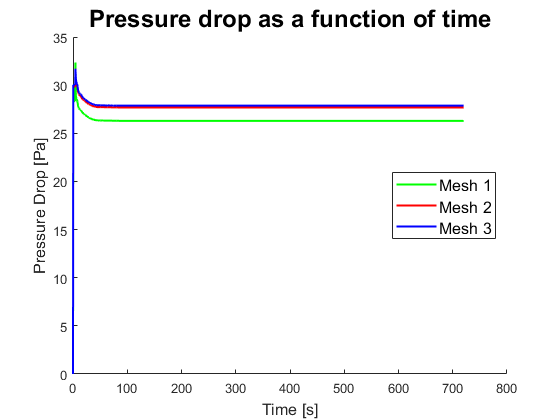
\includegraphics[width=\textwidth]{images/Meshsens/pres.png}
    \caption{Pressure}
    \end{subfigure}
    \begin{subfigure}{0.75\textwidth}\centering
    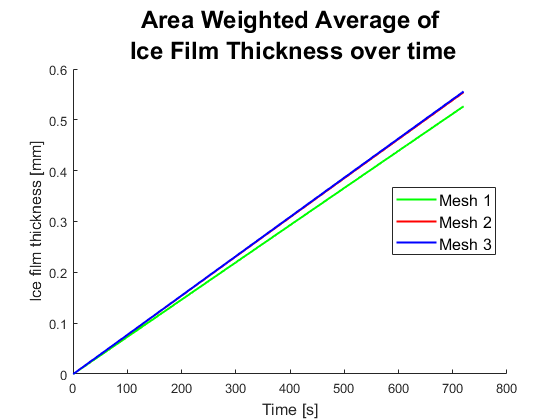
\includegraphics[width=\textwidth]{images/Meshsens/thick.png}
    \caption{Ice film thickness}
    \end{subfigure}
    \caption{Plots for mesh sensitivity - external flow}
    \label{fig:meshsens_out}
\end{figure}
For the internal flow simulation, which was a steady state case, the mesh sensitivity showed very close results. The graphical plot for the monitors can be seen in figure \ref{fig:meshsens_out}. The limits of the axes had to be tightened in order to observe a difference due to the closeness in the values of the monitors. Also, the mean value of the curve from the plots was considered for the sensitivity study. Based on the figures as well as table \ref{tab:meshsens_in}, it was decided to use the mesh with 16.05 million elements. {This can be justified based on the fact that there is effectively no deviation on almost doubling the element count.}
\begin{figure}[!ht]
    \centering
    \begin{subfigure}{0.75\textwidth}\centering
    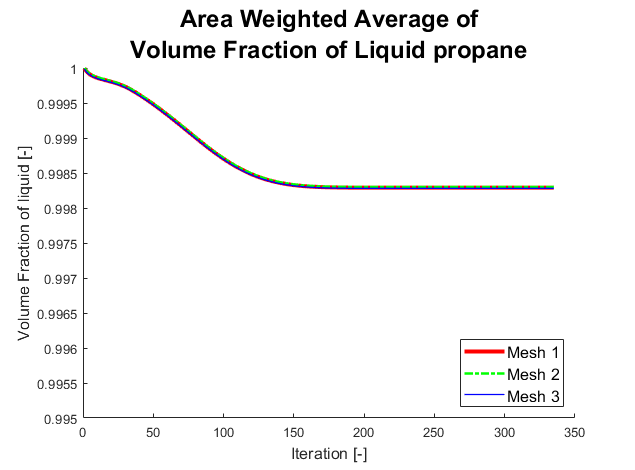
\includegraphics[width=\textwidth]{images/Meshsens/volfrac.png}
    \caption{Volume Fraction of Liquid Phase}
    \end{subfigure}
    \begin{subfigure}{0.75\textwidth}\centering
    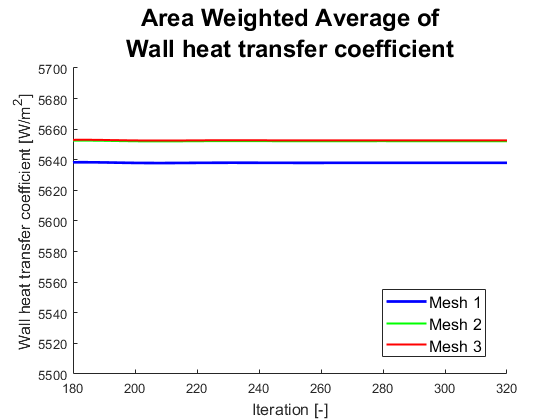
\includegraphics[width=\textwidth]{images/Meshsens/htc.png}
    \caption{Wall heat transfer coefficient}
    \end{subfigure}
    \caption{Plots for mesh sensitivity - internal flow}
    \label{fig:meshsens_in}
\end{figure}

\clearpage
\subsection{Solver Details}
\vspace{0.3cm}
Fluent offers two solver types for their simulations, those being the \textbf{Pressure Based} and the \textbf{Density Based} solvers.
\begin{itemize}
    \item \textbf{Pressure Based Solver}: This employs the projection method algorithm described by Chorin, J\cite{chorin}. This is defined in section 18.1.1 of the Fluent theory guide\cite{fluth}. The continuity of the velocity here is done through solving the pressure correction equation (in this case the equation of continuity). Ansys Fluent provides two solver algorithms, which are the segregated and coupled. In the segregated algorithm, the velocities in the x, y and z directions are solved sequentially, followed by the continuity equation. The mass flux, velocity and pressure are updated, followed by the solution of other properties such as energy, species, turbulence and other scalars.\\
    On the other hand, the coupled algorithm simultaneously solves the equations of momentum and continuity before updating the mass flux.%The differences between them are seen in figure \ref{fig:solv}.

    \item \textbf{Density Based Solver}: This is a coupled solver that solves the governing equations of continuity, momentum, energy and species transport simultaneously. This is an iterative procedure since the equations are non-linear.
\end{itemize}
    % \begin{figure}[!ht]
    %     \centering
    %     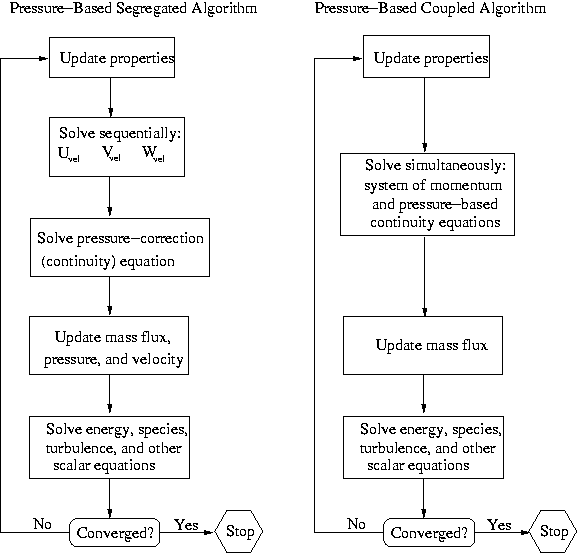
\includegraphics[width=0.8\textwidth]{images/pressure_based.png}
    %     \caption{Pressure-based solution algorithms\cite{fluth}}
    %     \label{fig:solv}
    % \end{figure}
    % \begin{figure}[!ht]
    %     \centering
    %     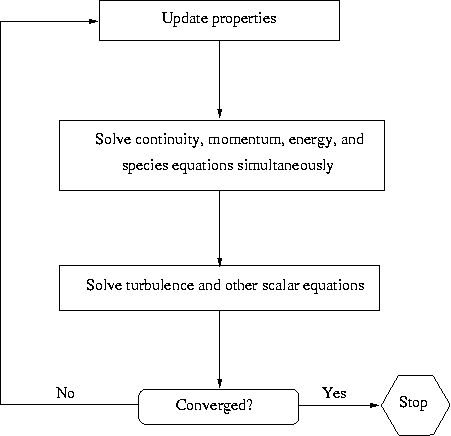
\includegraphics[width=0.8\textwidth]{images/density_based.png}
    %     \caption{Iterative flow for Density based solver\cite{fluth}}
    %     \label{fig:density}
    % \end{figure}
From section 36.1 of the Fluent User Guide, 2021\cite{flug}, the pressure based solver was developed mainly for incompressible and lightly compressible flows, whereas the density based solver was for high mach number flows. With improvements, both solvers can be used for a vast range of flows.

The Pressure based solver was used for the simulations, since the case is low-speed incompressible flow. The $k-\omega\ SST$ turbulence model was used for both simulations. This was considered the best choice as there were near wall effects that were needed to be captured, with a large part of the flow being in the free stream as well (section \ref{sec:turbmod}). The energy equation was also enabled in order to capture heat transfer. Based on the Fluent Theory guide and the Fluent User guide \cite{fluth}\cite{flug}, the following settings were considered for the simulations (as explained in section \ref{sec:theory}):
\begin{itemize}
    \item Coupled Solver with the following discretization schemes:
    \begin{itemize}
        \item Gradient : Least Squares Cell Based; Accuracy is on par with the Green-Gauss node based method (and more than the cell-based method) while being less computationally expensive.\cite{fluth}
        \item Density, Momentum, Turbulent Kinetic Energy, Energy, Specific Dissipation Rate: Second Order Upwind; As recommended in the theory guide to be a good balance between accuracy and computational speed\cite{fluth}\cite{flug}.
        \item Volume Fraction : First Order Upwind; Much faster to run than the available QUICK scheme, while not sacrificing on accuracy.
    \end{itemize}
\end{itemize}

 Additionally, monitor points were created in order to observe the simulation as it progressed. Monitors were based on report definitions created within Fluent, and were created for:

\begin{itemize}
    \item Average of film-thickness over the fins
    \item $\Delta P$ as in appendix \ref{app:presd}
    \item Static temperature average across inner wall (for internal simulation)
\end{itemize}

Additionally, the solution controls and under-relaxation factors were left at their Fluent specified defaults, which can be seen in table \ref{tab:relax}. These factors help reduce the oscillation of the residuals and enhance convergence. Using the default values specified in the software manual is considered good practice, as they are set to be optimal for a large number of situations. The values are to be lowered only in case of divergence of the solution (Section 36.3.2, Fluent User Guide\cite{flug}).
\begin{table}[!ht]
\centering
\caption{Table of under-relaxation factors used for the simulation}
\label{tab:relax}
\begin{tabular}{|l|l|}
\hline
\multicolumn{1}{|c|}{\textbf{Variable}} & \multicolumn{1}{c|}{\textbf{\begin{tabular}[c]{@{}c@{}}Under-relaxation\\  factor {[}-{]}\end{tabular}}} \\ \hline\hline
Pressure                  & 0.3 \\ \hline
Density                   & 1   \\ \hline
Body Forces               & 0.7 \\ \hline
Momentum                  & 0.7 \\ \hline
Volume Fraction           & 0.5 \\ \hline
Turbulent Kinetic Energy  & 0.8 \\ \hline
Specific Dissipation Rate & 0.8 \\ \hline
Turbulent Viscosity       & 1   \\ \hline
Energy                    & 1   \\ \hline
phase-1 h20               & 1   \\ \hline
\end{tabular}
\end{table}
\subsubsection{RGP Tables}
\vspace{0.3cm}
The study and the simulations involve phase change of the propane refrigerant. However, the software does not directly offer a way to simulate this phase change, since the Fluent material library does not provide separate materials for the liquid and vapour phases. Thus, Real Gas Property tables (from Fluent's REFPROP library) were used. This method entails using a few specified commands in order to obtain a table of properties of the fluid such as Density, Specific Heat, Thermal Conductivity and Viscosity as functions of Temperature and Pressure. The specific commands are included in Appendix \ref{app:code}.


\subsubsection{Surface Profiles}\label{sec:extflowsts}
\vspace{0.3cm}
According to the Fluent User's Guide \cite{flug} section 7.6.3, surface profiles are used to connect two separate simulations using the boundary profile in the result of one simulation as a boundary condition for another simulation. The available interpolation methods are: Constant, Inverse Distance and Least Squares. Since the surface element count was maintained the same for both the simulations in this study (see section \ref{sec:meshint}, constant (i.e. zero order) interpolation was used, as the solver would directly use the value at the cell. 

Therefore, based on figures $\ref{fig:newint}$ and $\ref{fig:newext}$, the inner wall of the pipe through with the refrigerant flows was used as the 'bridge' between the simulations, and surface profile data (i.e. the Heat Transfer Coefficient and Temperature) were exported from the internal simulation and used as a boundary condition for the same surface in the external flow simulation. The flowchart in figure \ref{fig:flowchart} shows the overall flow of the study.
\begin{figure}[!ht]
    \centering
    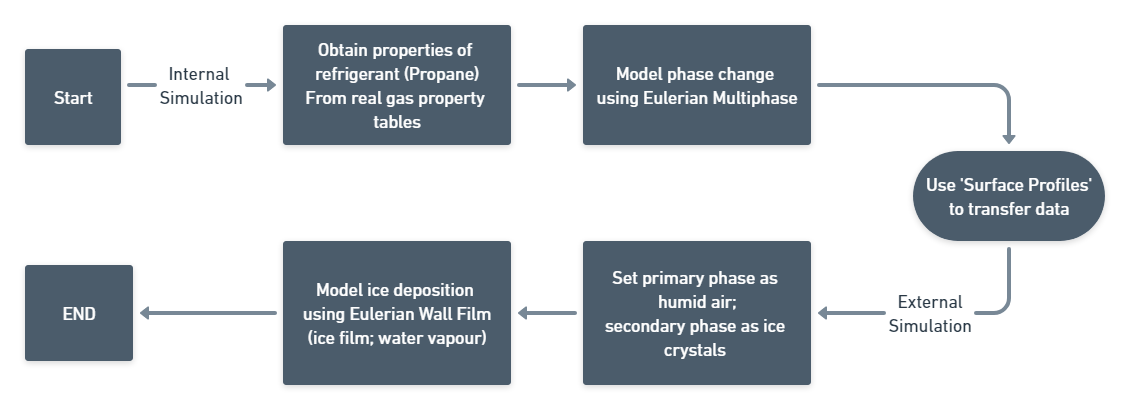
\includegraphics[width=\textwidth]{images/flowchart/propaner2.png}
    \caption{Flowchart depicting the simulation}
    \label{fig:flowchart}
\end{figure}
\pagebreak
\subsubsection{Internal Flow}\label{sec:internalsolv}
\vspace{0.3cm}
The internal flow simulation was initially set to have the same time-step as the the external flow simulation (of $0.5\ s$) in order to have the surface profile data at each instance in time. However, this led to a Courant Number of $10^4$, which would not satisfy the CFL condition\cite{cfl}. Thus, the simulation was conducted in a steady state situation. Additionally, the Pseudo-Transient method was enabled for faster convergence{\cite{fluth}}. The inlet was set as a mass-flow inlet with the value of the mass flow set at 0.028 kg/s as in the experimental scenario (0.252 kg/s from the experiment was for a capillary with 9 inlets into evaporator, leading to 0.028 kg/s for each circuit), at a pressure of 300 kPa. The inlet temperature was set to the evaporating temperature of $270K$ to match the manufacturer-specified evaporating temperature. RGP (Real Gas Property) tables were used to define the properties of the propane in its liquid and vapour states. Evaporation of propane was to be simulated. Based on the software manual\cite{flug}\cite{fluth} and section \ref{sec:mpflow}, the Eulerian Multi-Phase flow was enabled with the Evaporation/Condensation model and Lee Model enabled, as this was a direct situation for which the model was designed. The Multi-Phase model used has specifically designed for flows that involve boiling\cite{leemodel}. Convergence was considered to be achieved when all the residuals were stable and under $10^{-4}$ for multiple iterations. Fluent uses RMS deviation to calculate the residuals. Their tolerance value of $10^{-4}$ was considered to  achieve a sufficiently accurate solution\cite{convergence}. %The simulation was run until the residuals were stable and under $10^{-4}$.

\subsubsection{External Flow}\label{sec:externalsolv}
\vspace{0.3cm}
For the external flow simulation, since the fan was of the suction type, the inlet flow is assumed to {be turbulent with a uniform profile}.  In order to calculate the magnitude of velocity, the fan {properties} from the manufacturer were used. The relations shown in sectopm \ref{app:presd} were further used in expressions to compute the inlet velocity as a function of the ice thickness. This was done since the present study does not generate solid ice on the surface of the fin, and the predicted ice thickness is only mathematical, implying that the pressure drop does not change with time. The temperature of the inlet air was set to be $275K$ as in the experimental condition. For the walls, the roughness model for icing was enabled (as detailed in section \ref{sec:roughness}). The Eulerian Multiphase mixing model was enabled as discussed in section \ref{sec:mpflow}, as it was the best match according to the software manual\cite{flug}. The primary phase was set as a mix of air and water vapour, wherein the inlet also had a flow of water vapour equivalent to the relative humidity. The mole fraction of water was $0.0043$ at the inlet\footnote{Check Appendix \ref{app:rh}}. In order to have precise phase change at the walls, the Eulerian Wall Film model was enabled on the pipe surfaces and fins, solving the energy equation. This uses the Eulerian framework (section \ref{sec:mpflow}) to predict the creation of thin films on wall surfaces (see Chapter 22, Fluent Theory Guide\cite{fluth} and Chapter 29, Fluent User Guide\cite{flug}). Additionally, the phase change condition was also enabled. Convergence conditions were disabled and the time-step was set to 0.5 seconds. 

At this time-step, the Courant Number was calculated as\cite{cfl}:$$C=u\frac{\Delta t}{\Delta x}$$
Here, $u$ is the inlet velocity, $\Delta t$ is the time-step size and $\Delta x$ is the length of the smallest element (in this case, it was the cube root of the volume of the smallest element taken from fluent). In order to obtain a Courant Number of 1, the desired time step would be $4.16\times10^{-6}\ s$. This would be impractical, as the icing phenomenon takes a few minutes to be observed, and such a low time step would make the simulation take an exceedingly long time. The time step of $0.5\ s$ gives a CFL of $1.2\times10^5$ at a velocity of $5\ ms^{-1}$ (section \ref{app:presd}). It is known from previous studies that lower time-steps (and thus lower CFL numbers) didn't have any appreciable effect on the accuracy\cite{Afra} of the solution, and thus a time-step of $0.5\ s$ was selected. The simulation was run for 1440 time-steps (or 720 seconds) with 5 iterations per time-step.


%%%%%%%%%%%%%%%%%%%%%%%%%%%%%%%%  Chapter 4  %%%%%%%%%%%%%%%%%%%%%%%%%%%%%%%%%%%%%%%%%%%
\clearpage
\thispagestyle{empty}

\cleardoublepage

\thispagestyle{plain}

\section{Results}\label{sec:results}
\vspace{.6cm}
The following section presents the results obtained in the course of this study. The resultant contours and plots for both the internal and external simulations have been presented, namely the temperature and volume fraction contours for the internal flow, and the ice-film thickness contour for the external flow. Additionally, plots that show the ice-film growth along the fin surface are also presented.

\subsection{Internal Flow Simulation}
\vspace{0.3cm}
For the internal flow simulation, figure \ref{fig:in_restemp} shows the contours of the wall temperature.  It is seen that the temperature variation is almost negligible, and almost a constant $270K$, which is the evaporating temperature of the refrigerant. Additionally, figure \ref{fig:in_volfrac} shows the volume fraction of the liquid phase at the walls plotted against the distance from the inlet. A value of 1 is pure liquid, while a lower value is a mixture of the liquid and vapour phases. This data was obtained by taking a path-lines from the inlet to the outlet along the walls, and averaging them to get a single value at each location.
\begin{figure}[!ht]
    \centering
    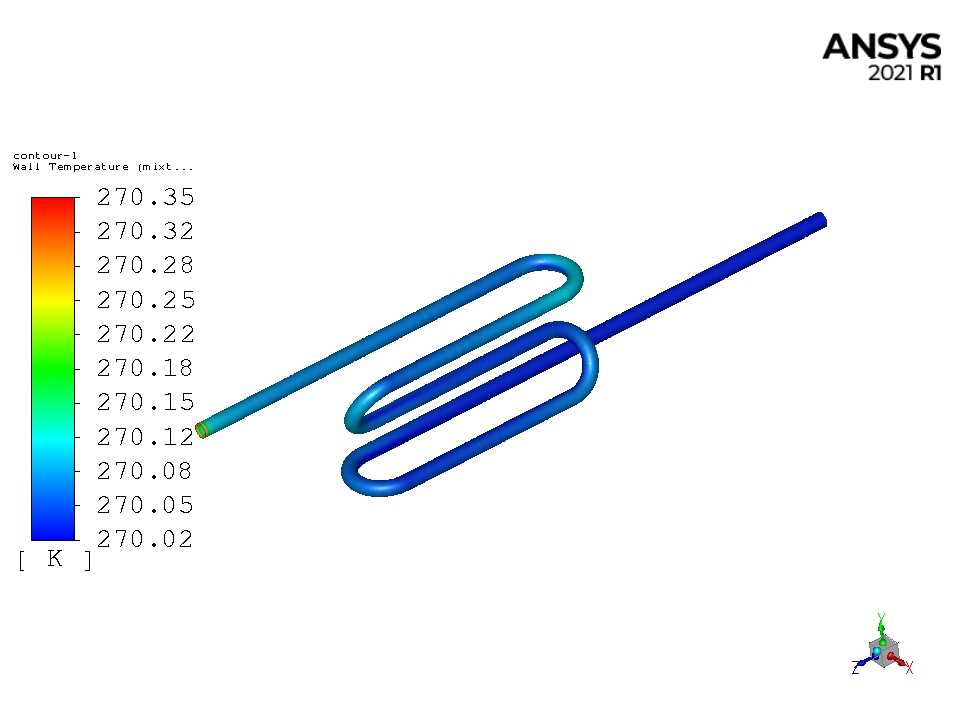
\includegraphics[width=0.8\textwidth]{images/result_inner_temp.jpg}
    \caption{Inner wall temperature contours, showing a constant wall temperature of $~270\ K$ along the entire length of the tube}
    \label{fig:in_restemp}
\end{figure}

% \begin{figure}[H]
%     \centering
%     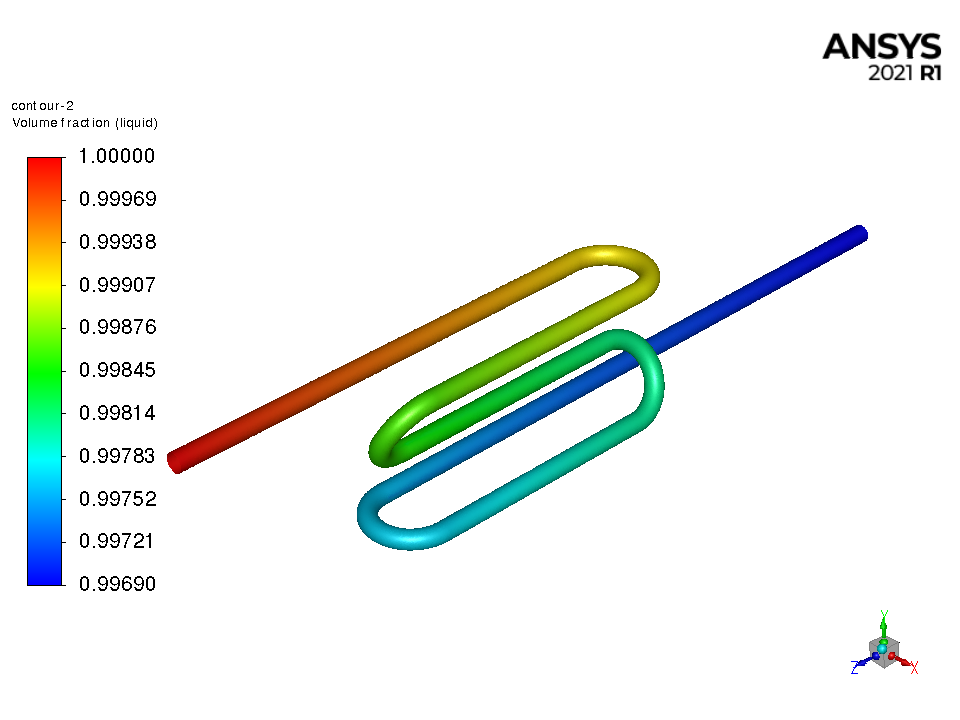
\includegraphics[width=0.8\textwidth]{images/result_inner_vol.png}
%     \caption{Volume Fraction contours of liquid phase along the wall}
%     \label{fig:in_volfrac}   
% \end{figure}

\begin{figure}[H]
    \centering
    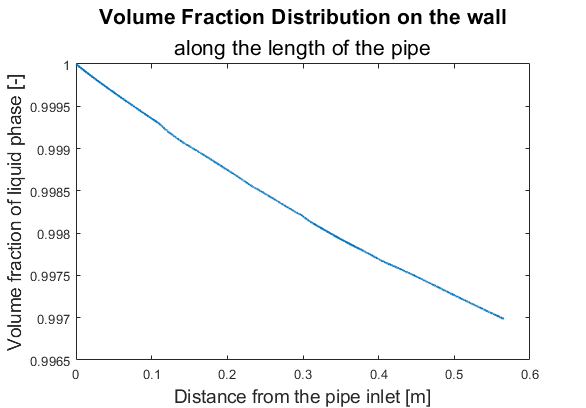
\includegraphics[width=0.8\textwidth]{images/resgrph/pipe_length.png}
    \caption{Volume Fraction of the liquid phase (at the wall) plotted against the distance from the inlet of the pipe}
    \label{fig:in_volfrac}   
\end{figure}

\subsection{External Flow Simulation}
\vspace{0.3cm}
The contours of ice film thickness obtained after running the simulation for the specified 720 seconds (12 minutes) can be seen in figure \ref{fig:out_res1}. The contour shows that a majority of the ice is deposited on the side of the fins (and pipes) that is directly facing the oncoming air.

\begin{figure}[!ht]
    \centering
    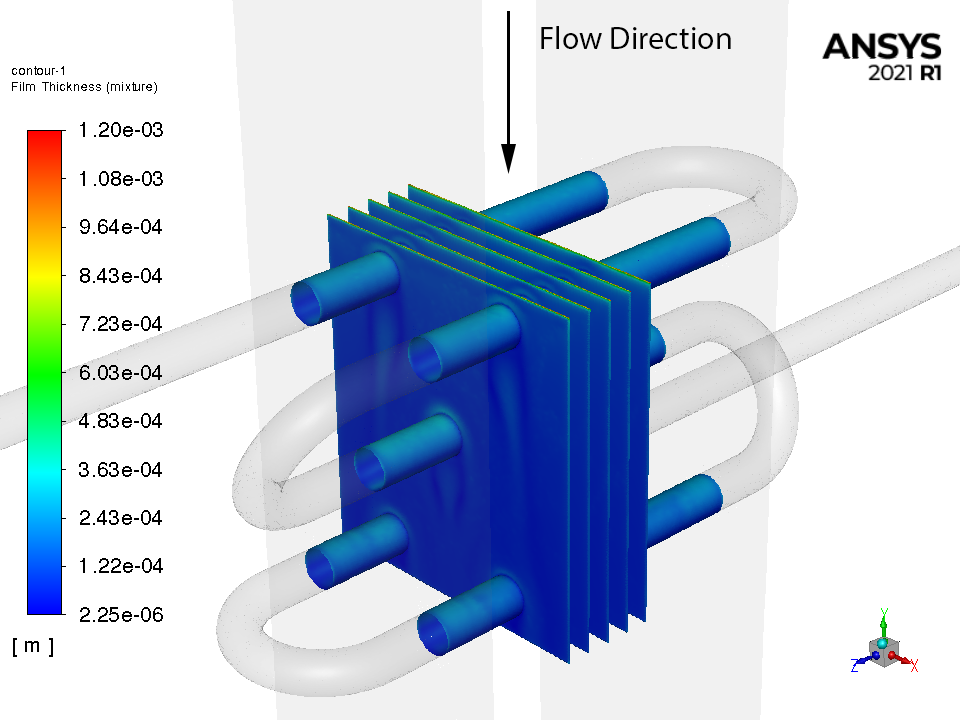
\includegraphics[width=0.8\textwidth]{images/fullcontour.png}
    \caption{Ice film thickness on the fins and pipes}
    \label{fig:out_res1}   
\end{figure}

However, any ice growth in the y direction doesn't block the flow, and therefore, doesn't contribute much to the pressure loss. Thus, transverse (ZX) planes were taken at 3 separate locations on the fins (as can be seen in figure \ref{fig:findata}). The distances from the top of the fin to those planes are $0.2\ mm$, $10\ mm$ and $30\ mm$ respectively The average of final ice film thickness (after $720\ s$) at those planes from both faces of each fin were plotted against the location along the x axis. This can be seen in figure \ref{fig:filmthickx}. It can be seen that the magnitude of ice thickness in the z direction (which directly contributes to the pressure loss of the oncoming air) drops significantly the lower we move along the fin.  %Additionally, a second figure, \ref{fig:out_res2}, can also be seen, which is the contours of the film thickness on an iso-surface at the first cell height on the vertical fin wall (parallel to the  flow) overlaid on the geometry. To qualify these results, 
Based on figure $\ref{fig:filmthickx}$, the contour of ice film thickness on Plane 1 is shown in figure $\ref{fig:out_res2}$. It can be observed from this (and figure $\ref{fig:filmthickx}$) that the thickness is strongly affected by the presence of a pipe. Additionally, the pressure drop caused by the evaporator geometry as a function of time can be seen in figure $\ref{fig:press}$. This plot shows that after stabilization of the flow, the pressure drop is mostly constant. This indicates that the ice growth being predicted is mathematical, and therefore does not affect further iterations of the solver. The software isn't depositing solid ice on the surface, but is only predicting how much ice would be deposited at that time.

\begin{figure}[!ht]
    \centering
    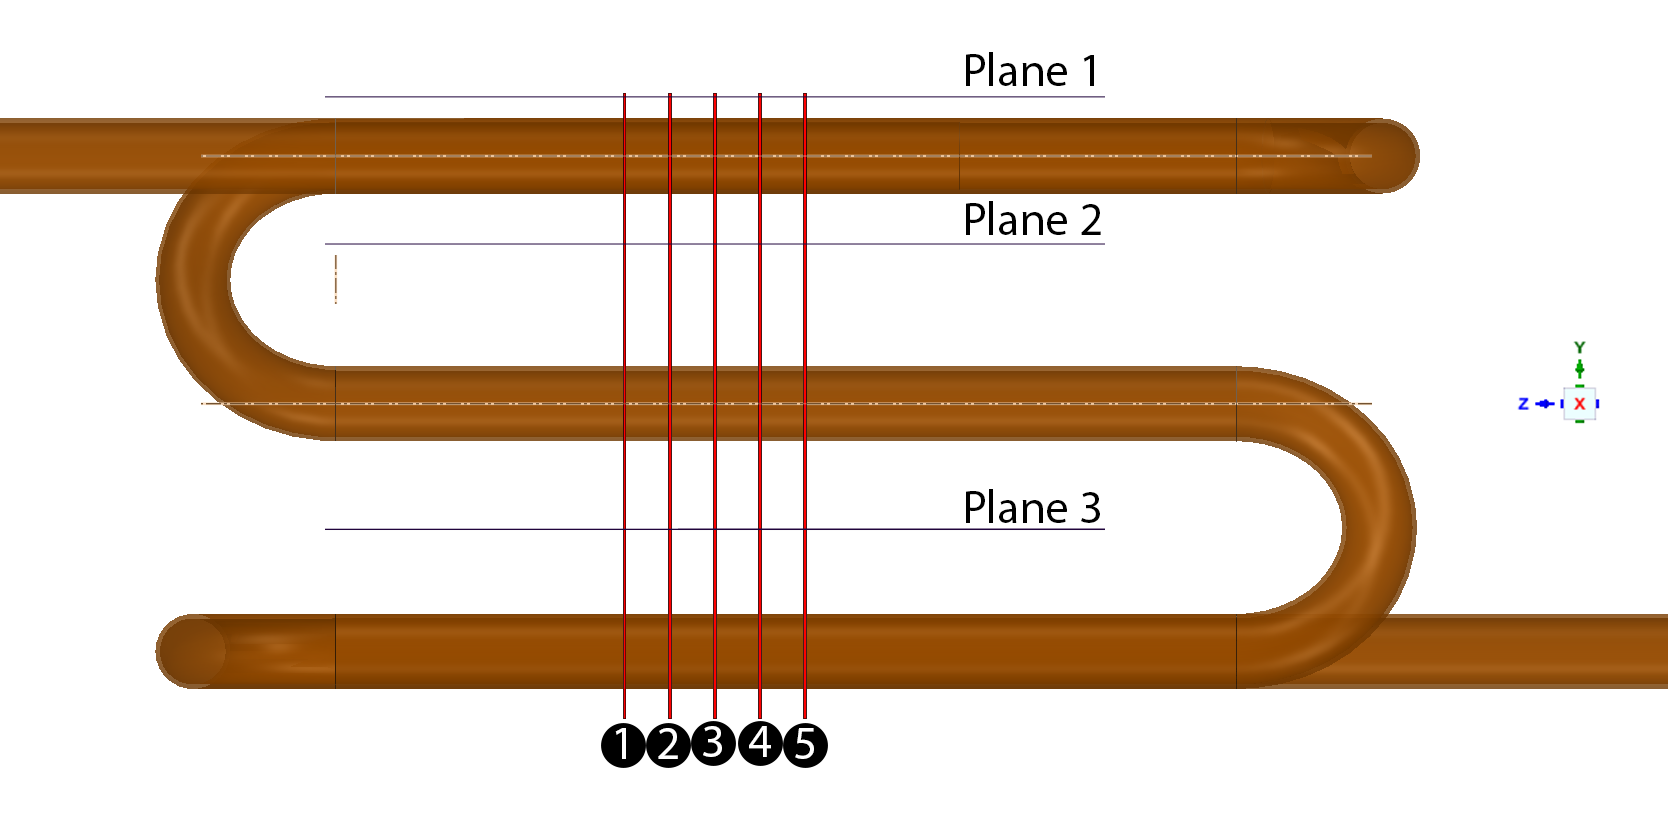
\includegraphics[width=0.8\textwidth]{images/planes2.png}
    \caption{Location of transverse planes}
    \label{fig:findata}
\end{figure}

\begin{figure}[!ht]
    \centering
    \begin{subfigure}{0.49\textwidth}
    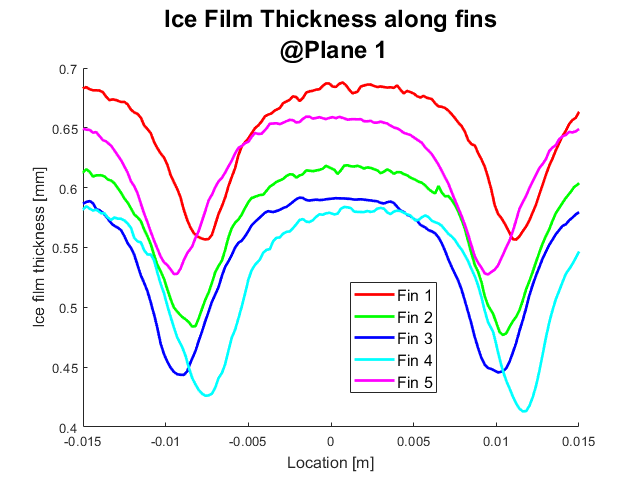
\includegraphics[width=\textwidth]{images/resgrph/plane1.png}
    \caption{Plane 1}
    \label{fig:filmthickx_1}
    \end{subfigure}
    \begin{subfigure}{0.49\textwidth}
    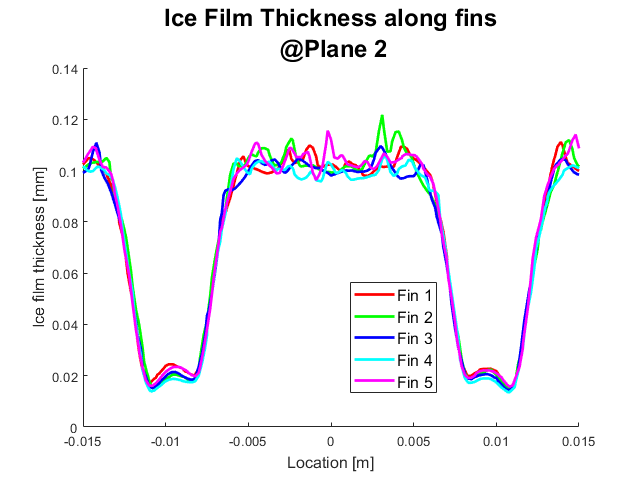
\includegraphics[width=\textwidth]{images/resgrph/plane2.png}
    \caption{Plane 2}
    \label{fig:filmthickx_2}
    \end{subfigure}
    \begin{subfigure}{0.49\textwidth}
    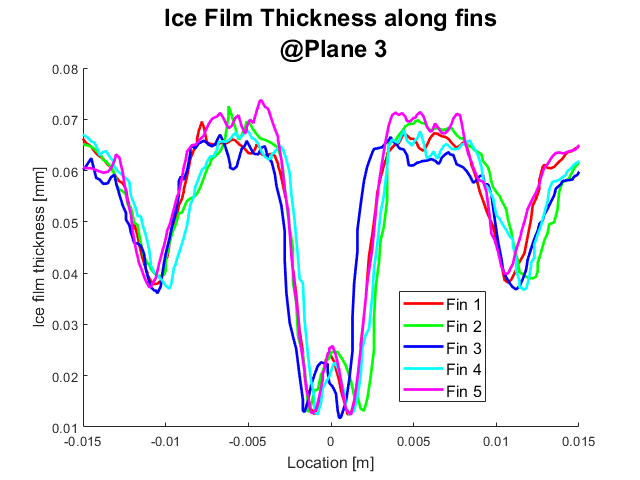
\includegraphics[width=\textwidth]{images/resgrph/plane3.png}
    \caption{Plane 3}
    \label{fig:filmthickx_3}
    \end{subfigure}
    \caption{Ice fin thickness across the fin at various planes}
    \label{fig:filmthickx}
\end{figure}

\subsection{Model Validation}\label{sec:valid}
\vspace{0.3cm}
The comparison plot of the experimental value of ice thickness against the obtained CFD results is included in figure \ref{fig:comparison}.  {The CFD results were obtained by taking an area-weighted average of the film thickness on Plane 1 as referred above}. Additionally, the experimental curve is a fitted polynomial (as in figure \ref{fig:expchart}). It should be noted that the experiment already had some measure of icing already present initially, which is the reason that the experimental curve has an intercept. It can also be seen that the experimental results and CFD results have differing slopes, and that the ice buildup in the experimental case is slightly slower than in the CFD case. The reason has been explained in section \ref{sec:disc}.
\begin{figure}[!ht]
    \centering
    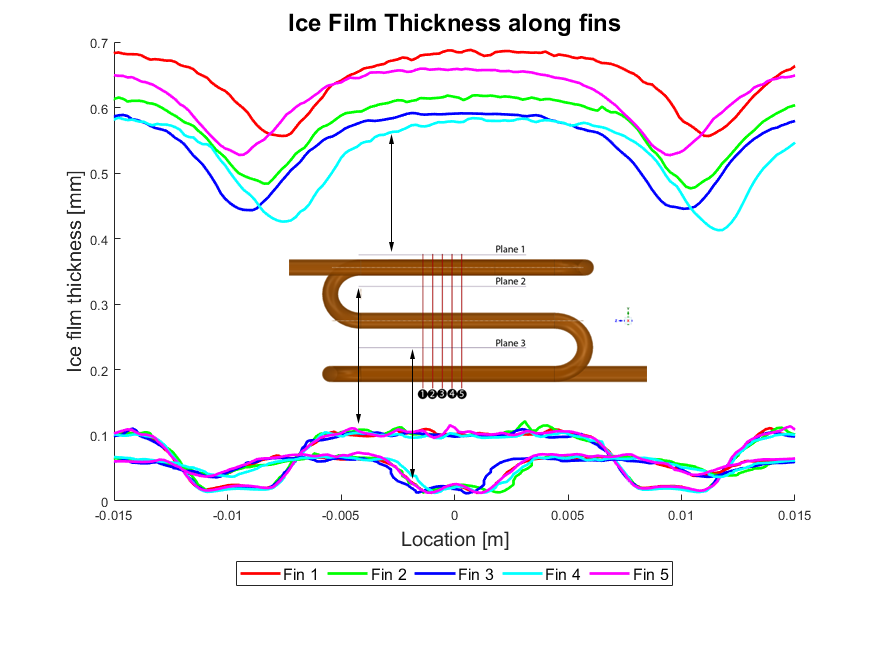
\includegraphics[width=0.8\textwidth]{images/resgrph/planar.png}
    \caption{Combined plots for all three planes (ref. figures \ref{fig:findata} and \ref{fig:filmthickx})}
    \label{fig:planars}
\end{figure}

\begin{figure}[!ht]
    \centering
    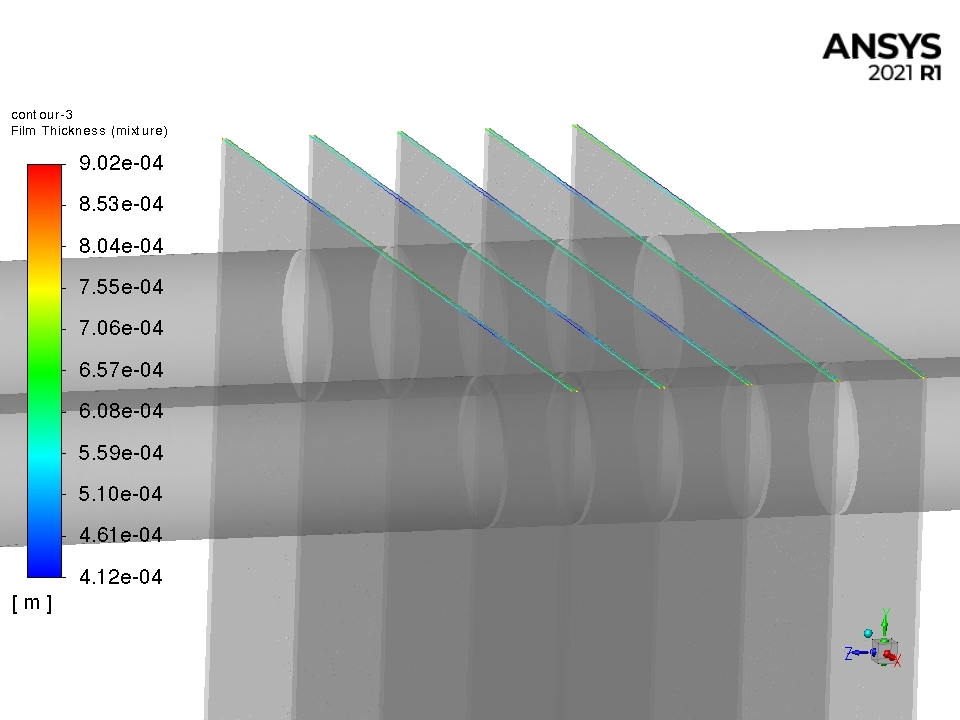
\includegraphics[width=0.8\textwidth]{images/linecont.jpg}
    \caption{Ice film thickness on the iso-surface at plane 1, overlaid with geometry}
    \label{fig:out_res2}   
\end{figure}

\begin{figure}[!ht]
    \centering
    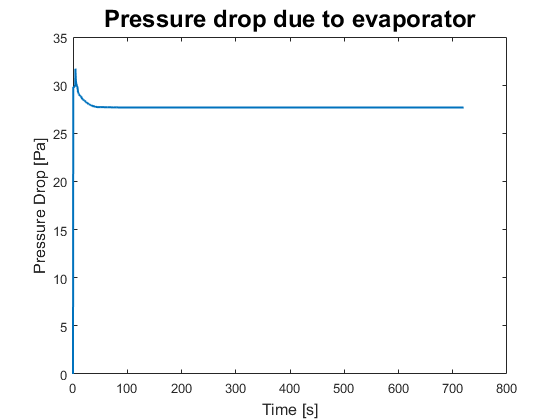
\includegraphics[width=0.7\textwidth]{images/pressure_drop.png}
    \caption{Pressure drop as a function of simulation time}
    \label{fig:press}
\end{figure}
\begin{figure}[!ht]
    \centering
    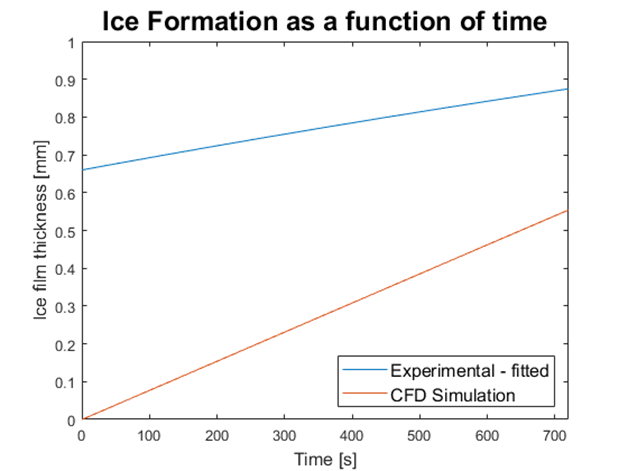
\includegraphics[width=0.8\textwidth]{images/result_comparison.png}
    \caption{Ice film thickness obtained in the CFD calculation compared against the experimental result}
    \label{fig:comparison}
\end{figure}


%%%%%%%%%%%%%%%%%%%%%%%%%%%%%%%%  Chapter 5  %%%%%%%%%%%%%%%%%%%%%%%%%%%%%%%%%%%%%%%%%%%
\clearpage
% \thispagestyle{empty}
% \cleardoublepage
\thispagestyle{plain}
\section{Discussion} %and Limitations}
\label{sec:disc}
\vspace{.6cm}

The experimental procedure followed in the beginning of this study uses a climate chamber to simulate the conditions that the heat pump would face when being used. In order to measure the properties, sensors were installed at various locations as necessary to measure the properties such as the pressure drop over the evaporator, the evaporator pressure and so on. Since ice that is deposited over the fins would block the path of the flow over the evaporator, further ice build up would cause a drop in pressure across the evaporator. Thus, the ice thickness was calculated by using an empirical formula that was developed by the company that related the thickness of the ice being deposited to the pressure drop. While this was considered to be accurate based on previous findings at the company, accuracy would definitely be improved by using an ultrasound depth sensor to measure the ice thickness.

In order for the software to simulate the condition as required, the case was split between the internal flow (which was the refrigerant within the pipe) and the external flow (which was the ice deposition simulation). This simulation need not have been performed, however, and the boundary condition for the external flow could have been set to a constant value of temperature and heat transfer throughout (instead of the current surface profile condition). While this would reduce simulation time, it would also mean that some intricacies would not be observable. As an example, figure \ref{fig:in_volfrac} shows that there is a gradual evaporation in the fluid as it moves along the pipe. This causes a difference in the performance of the evaporator, as the vapour and liquid refrigerant have different thermal properties. As more of the refrigerant evaporates, its ability to take away heat reduces. Thus, even though there is a greater time investment, the simulation of the refrigerant provides for improved accuracy in the overall result.

In the course of the internal flow simulation, in order to effectively model the phase change of the refrigerant (propane in this case), the thermodynamic material models for the vapour phase and liquid phase must be defined accurately. This was done with the help of the Refrigerant Properties Database by the US National Institute of Standards and Technology (NIST). Since the properties would not be constant throughout on account of phase change, there would have to be a way to provide the solver with a table of the properties for both the phases. The way to do this was by using the Real Gas Property tables for these fluids. These tables contain properties such as density, specific heat and viscosity at different combinations of pressure and temperature between a set range. These were generated as described in appendix \ref{app:code}, and then incorporated within the solver. The solver then used this table of data to then calculate the fluid properties as needed. This was not required for the external flow simulation as the data for the three phases of water are already present in the software material database.

Considering the results of the internal flow simulation, figure $\ref{fig:in_volfrac}$ shows the volume fraction of the refrigerant at the walls is decreasing on moving downstream of the inlet. Additionally, figure $\ref{fig:in_restemp}$ shows a constant temperature along the wall of $270K$, which matches with the evaporator data provided by the manufacturer. Looking at the results, it can be seen that as the refrigerant passes through the pipe, it is changing phase. Since the wall temperature matches the inlet condition of fluid ($270\ K$), it indicates that the phase change is isothermal, and thus the refrigerant is undergoing latent heating. This is the principle behind the working of an evaporator, and the figures show that the phenomenon is captured well.

Considering the results of the external flow, figure \ref{fig:out_res1} was obtained after running the simulation for 720 seconds. It shows that the maximum amount of ice growth has happened in the region that is directly facing the incoming air, and decreases as we move further downstream along the fin. This is physically realistic, and increases confidence in the simulation. Figure \ref{fig:filmthickx} shows the variation in ice film thickness along the surface of the fin in both the stream-wise and transverse directions. It can be that the pipes have an effect not just downstream to them, but also upstream. These pipes behave like a cylindrical body in the free stream flow, and looking at the aerodynamic effects of flow around a cylinder\cite{ketticylinder}, it can be seen that there is a small stagnation region just ahead of the cylinder. Thus, it shows that the evaporator pipes have a blocking effect on the flow\cite{longblocker}, causing the ice-deposition to be concentrated just upstream the pipe, while reducing it at slightly larger distances. This can also be observed to a slight degree in figure \ref{fig:out_res1}. On taking the graphs in figure \ref{fig:filmthickx} into account, it can be observed that the wake regions of the cylinder have a lower amount of ice being deposited. This leads to an interesting observation that the ice deposition on the fin surface increases as the velocity of the air flowing over it is increased, since the mass flow rate of the water vapour is increased.

Additionally, it can be observed from figure \ref{fig:filmthickx_1} that there is a larger amount of ice that is deposited on the fins at the periphery for this plane. Since the gap between the fins is quite small, a majority of air flows around the fins. Thus, for a majority of air flow, the block of fins can be considered to be a bluff body in a channel. From studies on the behaviour of bluff bodies\cite{bluffbody1}\cite{bluffbody2}, the flow accelerates near the leading edge of the bluff body due to constriction in flow area. Since fin number 5 is further from the wall, the velocity increase is lower and thus the slightly lower thickness of the ice film on this fin. These results can be used in further studies to optimize the distance between the evaporator fins and the nearest wall, as well as the fin pitch. This can minimise the ice deposition the ice deposition as well as improve the aerodynamic characteristics, which in turn can improve the performance of the evaporator.

Figure \ref{fig:planars} shows a comparison between the ice film thickness plots among the three planes. It can be observed that there is a marked difference between the ice thickness near the leading edge of the fins than the rest of the surface. Thus, it can be inferred that the majority of the pressure drop (due to ice) caused would be due to buildup near the leading edge. Since the flow is in the negative y direction (see figure \ref{fig:findata}), it is prudent to consider growth in the transverse (i.e. $\pm$z direction). Thus, the average ice film thickness at plane 1 was used as a reference observe the ice growth. Figure \ref{fig:out_res2} shows the contour, and is a visual representation of what can be observed from the plot in figure \ref{fig:filmthickx_1}.%  was used as a reference to  in the direction perpendicular to the air-flow, which would be the major cause for pressure drop in the real world. 

From section \ref{sec:valid} and subsequently figure \ref{fig:comparison}, the graph for the experimental results and the simulated results are in the same order of magnitude. It should be noted, however, that the experiment already had a significant amount of ice already present on the evaporator fins. According to studies that have been conducted\cite{heatexchdiff}, the rate of ice deposition reduces as the ice builds up. Thus, it is realistic that the slope of the CFD simulation results is seemingly higher than the experimental results. Further reasons for the deviation and the limitations of the conducted study can be found in section \ref{sec:limit} below.

\clearpage
\section{Limitations}\label{sec:limit}
\vspace{.6cm}

The major point to note is that the geometry has been simplified. This means that there is simply less area of the evaporator that is in contact with the air to frost over. As discussed in section \ref{sec:disc}, presence of ice at the beginning of the experiment also would have impacted the results, and reduced the slope of the curve.

Additionally, one of the major points of simplification was that the internal flow simulation was a steady state simulation and as such, the wall temperature and heat transfer coefficient along the pipe's inner wall were constant (when exported to the external flow). Since the simulations were only linked in one way (i.e. data from internal was used in the external simulation), it wasn't possible to take into account the reduction in heat transfer due to the surface being covered in frost. A way forward would be an iterative procedure; the heat transfer profile on the evaporator and pipe outer walls would be used as the boundary condition for the internal flow simulation. A flowchart for the same can be represented as:
\begin{figure*}[!ht]
    \centering
    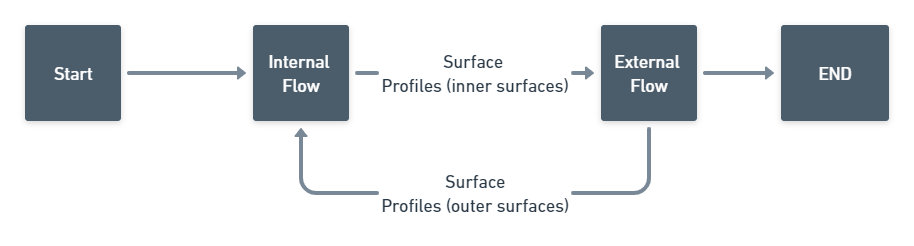
\includegraphics[width=.8\textwidth]{images/flowchart/BC Flow.png}
\end{figure*}

Iterating the study in this way would ensure that there was a parity between the simulations and improve the confidence in the simulations.

Choosing to simulate the internal flow as a transient simulation for future studies would no doubt improve the quality of the results, as the surface profiles could be exported at the required instances in time. This would ensure that the heat transfer coefficient data provided to the external flow simulation is not constant, but a function of time. This would require the use of a User Defined Function or UDF (as detailed in the Fluent UDF Manual\cite{fludf}). However, it would then be necessary to match the time-steps for the internal and external simulations, which would exponentially increase the required computational resources.\\

A consequence of the models used (as in sections \ref{sec:theory} and \ref{sec:method}) is that the ice film calculated by Fluent (which can be seen in figure \ref{fig:out_res1} is purely mathematical, without changing the surface composition (and thus the flow field around the fins). This is also corroborated by the pressure remaining constant through most of simulation as seen in figure \ref{fig:press}.\\
As a consequence, the velocity change that would be caused by a pressure drop needs to be mathematically calculated and set as a boundary condition. This, while possible (see Appendix \ref{app:presd}, figure \ref{fig:projvel}), is a less than ideal substitute for actual pressure drop, and would also reduce the amount of water vapour that enters the domain in the first place, thus reducing the overall rate and amount of ice growth.\\
A way to get around this would be to use a constantly adapting mesh that changes based on the calculated ice thickness as detailed in section 11.6 of the Fluent User Guide \cite{flug} based on the equations as detailed in section 3.2 of the theory guide \cite{fluth}. Consequently, the pressure drop would be captured realistically and in a physically accurate sense.
% As a consequence of the models used, the film that is calculated by Fluent (seen in figure \ref{fig:out_res1}) is purely mathematical and there isn't any change in the overall flow field. This is also corroborated by figure \ref{fig:press}. This leads to the fact that the inlet velocity needs to be reduced via an expression, thereby adding a measure of uncertainty to the conducted study. While the equations have been subject to testing at Bosch, they're no substitute for actual simulations.\\

Despite these limitations, the results of the experimental and CFD simulations are in the same order of magnitude, and the study can be taken as a basic, formative step towards developing a more comprehensive model.

%%%%%%%%%%%%%%%%%%%%%%%%%%%%%%%%  Chapter 6  %%%%%%%%%%%%%%%%%%%%%%%%%%%%%%%%%%%%%%%%%%%
\clearpage

% \thispagestyle{plain}

\section{Conclusions and Future Scope}

\vspace{.6cm}

A basic CFD methodology was developed in order to predict the icing and the thickness of the ice-film layer on the surface of the evaporator fins. This developed methodology is capable of predicting the icing based on the refrigerant within the pipes, and the atmospheric condition externally. Even with a scaled down geometrical configuration, the results of the CFD simulation are in the same order of magnitude as the experimental results. This shows that with a few tweaks, the simulated model could be equivalent to experimental studies. The internal simulation effectively predicts that there is evaporation along the walls of the evaporator pipes and this happens at the evaporating temperature as obtained through experimentation. The external flow is capable of mathematically capturing the ice film thickness.\\

While there are a few limitations within the model, it can be considered to be a solid foundation to the development to a complete CFD model. A few steps could be taken, however, to take it in the right direction. The first step would be to run the internal simulation as a transient case at a CFL of unity. This would let the data be collected at each instance in time. This would be coupled to an iterative process of using profiles from the internal and subsequently the external simulation till the solutions converge and the final profiles can be taken to be identical to the real-world data. While this step is time-consuming, it gives transient data for the internal pipe flow, which makes the heat transfer in the system to be more representative of the real world. Doing this also makes it so the model is ready to use with maximum accuracy for non-frosting conditions. It would be capable of predicting the thickness of the water film on the surface of the fins without a lot of hassle. 

An additional instance where this model could be bettered is by using a dynamic mesh in the regions where there is frosting (in the external flow case). A dynamic mesh changes each iteration with new information, which in the study would be the thickness of the ice layer at each location. This enables the real pressure drop to be calculated, thereby avoiding the use of empirical relations in the CFD study. Performing this step would lead to a direct comparison between the CFD model and the experimental case while also providing more representative results.

% %%%%%%%%%%%%%%%%%%%%%%%%%%%%%%%%  Chapter 7  %%%%%%%%%%%%%%%%%%%%%%%%%%%%%%%%%%%%%%%%%%%
% \clearpage
% \thispagestyle{empty}

% \cleardoublepage

% \thispagestyle{plain}

% \section{Future Scope}

% \vspace{.6cm}


%%%%%%%%%%%%%%%%%%%%%%%%%%%%%%%%  References %%%%%%%%%%%%%%%%%%%%%%%%%%%%%%%%%%%%%%%%%%
\clearpage
\thispagestyle{empty}

\cleardoublepage

\thispagestyle{plain}%\addcontentsline{toc}{section}{References}

\printbibliography[heading=bibintoc]
% \bibliography{references}
% \bibliographystyle{vancouver}
%\putbib[references]
%\end{bibunit}
%%%%%%%%%%%%%%%%%%%%%%%%%%%%%%%%  Appendix  %%%%%%%%%%%%%%%%%%%%%%%%%%%%%%%%%%%%%%%%%%%
\clearpage
\thispagestyle{empty}

\cleardoublepage

\thispagestyle{plain}

%\appendix
% \begin{bibunit}

%\section{Appendix}

\appendix
\newrefsection
% \addcontentsline{toc}{section}{Appendices}


\section{Appendix}

\vspace{.6cm}


\subsection{Generating RGP Tables}\label{app:code}
\vspace{.3cm}
 The method to generate the RGP tables is specified in the Fluent Beta Manual 2021\cite{flubeta}. Initially, it is required to navigate to the directory where Ansys is installed, via opening the Command Prompt/Terminal and entering:
\begin{verbatim}
    %AWP_ROOT211%\SystemCoupling\bin\systemcoupling.bat   
\end{verbatim}
This opens a Python shell at the location. The commands used to specifically generate the propane RGP tables for the conducted study were as follows:
\begin{lstlisting}[language=python,numbers=none]
import pyExt.RefProp as arp
fluidsPath = arp.getFluidsPath()
mat = arp.RefPropLib()

fluidList = ['fluids/propane.fld']
#replace propane with required fluid
mat.setup(fluidsPath, fluidList)

Tmin = 240.0
Tmax = 400.0
Pmin = 100000.0
Pmax = 25000000.0 
#Range of values over which RGP table is required

proprgp = arp.RGPSettings("C3H8", Tmin, Tmax, Pmin, Pmax, 1.0e-4, arp.ADAPT_AUTO_TP)
arp.generateRGPfile("C3H8-RGP.rgp", proprgp) 
#The maximum allowable error is 1e-4
\end{lstlisting}
This generates a `.rgp' file at the location where the command was run. Since this is usually in the C:$\backslash$ Drive on Windows systems, Admin access is required to obtain the generated file. The list of available fluids in Fluent's REFPROP database can be found in the Fluent User's guide section 8.16.4.2\cite{flug}.

\subsection{Relative Humidty Calculation}\label{app:rh}
\vspace{0.3cm}
Relative Humidity is defined as the ratio of the partial pressure of water vapour to the saturation pressure at that temperature. A special formulation\cite{its90} was used to calculate the saturation temperature. This formulation (for the case of water vapour over ice between 0 and 100$\degree$ C can be seen in equation \ref{eq:rhform} below:
\begin{equation}\label{eq:rhform}
    \ln e_{s}=\sum_{i=0}^{6} g_{i} T^{i-2}+g_{7} \ln T
\end{equation}
Where $e_s$ is the saturation vapour pressure, and $T$ is the temperature in Kelvin. For the ITS-90 scale, the constants $g_0$ through $g_7$ are given as:
$$\begin{array}{l}
\mathrm{g}_{0}=-2.8365744 \times 10^{3} \\
\mathrm{g}_{1}=-6.028076559 \times 10^{3} \\
\mathrm{g}_{2}=1.954263612 \times 10^{1} \\
\mathrm{g}_{3}=-2.737830188 \times 10^{-2} \\
\mathrm{g}_{4}=1.6261698 \times 10^{-5} \\
\mathrm{g}_{5}=7.0229056 \times 10^{-10} \\
\mathrm{g}_{6}=-1.8680009 \times 10^{-13} \\
\mathrm{g}_{7}=2.7150305
\end{array}$$
Once the saturation pressure is known, the relative humidity can be used to then calculate the partial pressure of the water as:$$RH=\frac{p_w}{p_{sat,w}}\implies p_w=RH\cdot p_{sat,w}$$
Subsequently, the mole fraction of water can be calculated as:
$$y=\frac{p_w}{p_{ambient}}$$
% \subsubsection{Heading level 3}

% \noindent
% \blindtext[1] \\

% \noindent
% \textbf{Heading level 4}
% \vspace{.3cm}

% \noindent
% \blindtext[1]


\clearpage

%-----------------------------------------------------------------------------------



%%%%%%%%%%%%%%%%%%%%%%%%%%%%%%%%  Appendix References  %%%%%%%%%%%%%%%%%%%%%%%%%%%%%%%%%%%%%%%%%%%

\printbibliography
% \putbib[references]
% \end{bibunit}

\end{document}
